%\documentclass[12pt,modern,twocolumn,tighten]{aastex63}
\documentclass[12pt,twocolumn,linenumbers]{aastex63}
%\documentclass[12pt,modern,twocolumn,tighten,linenumbers,trackchanges]{aastex63}
%\documentclass[12pt,twocolumn,tighten,linenumbers]{aastex63}
%\documentclass[12pt,twocolumn,tighten,trackchanges]{aastex63}
\usepackage{amsmath,amstext,amssymb}
\usepackage[T1]{fontenc}
\usepackage{apjfonts}
\usepackage[figure,figure*]{hypcap}
\usepackage{graphics,graphicx}
\usepackage{hyperref}
\usepackage{natbib}
\usepackage[caption=false]{subfig} % for subfloat
\usepackage{enumitem} % for specific spacing of enumerate
\usepackage{epigraph}

\renewcommand*{\sectionautorefname}{Section} %for \autoref
\renewcommand*{\subsectionautorefname}{Section} %for \autoref

\newcommand{\cn}{Cep-Her complex} % cluster name
\newcommand{\sysone}{Kepler-1627} % star system name (binary)
\newcommand{\stone}{Kepler-1627 A} % star system name (binary)
\newcommand{\plone}{Kepler-1627 Ab} % planet name
\newcommand{\systwo}{Kepler-1643} % star system name (binary)
\newcommand{\sttwo}{Kepler-1643} % star system name (binary)
\newcommand{\pltwo}{Kepler-1643 b} % planet name
\newcommand{\systhree}{KOI-7368} % star system name (binary)
\newcommand{\stthree}{KOI-7368} % star system name (binary)
\newcommand{\plthree}{KOI-7368 b} % planet name
\newcommand{\sysfour}{KOI-7913 } % star system name (binary)
\newcommand{\stfour}{KOI-7913 A} % star system name (binary)
\newcommand{\plfour}{KOI-7913 Ab} % planet name

\newcommand{\clusterage}{$38^{+6}_{-5}$\,Myr} % 

\newcommand{\npms}{1097} % 20220311_Kerr_SPYGLASS205_Members_All.csv

%
% Symbols
%
\newcommand{\kms}{\,km\,s$^{-1}$}
\newcommand{\mkms}{{\rm \,km\,s^{-1}}}  % math mode
\newcommand{\ms}{\,m\,s$^{-1}$}
\newcommand{\bpmrpo}{(G_{\rm BP}-G_{\rm RP})_0}
\newcommand{\bpmrp}{G_{\rm BP}-G_{\rm RP}}

%% Reintroduced the \received and \accepted commands from AASTeX v5.2.
%% Add "Submitted to " argument.
\received{\today}
\revised{---}
\accepted{---}
%\submitjournal{AAS Journals}
\shorttitle{Kepler Mini-Neptunes in Cep-Her}

\begin{document}

\title{
  A Trio of 40 to 50 Million Year Old Mini-Neptunes from Kepler, TESS, and Gaia
}

%\suppressAffiliations
%\NewPageAfterKeywords
\correspondingauthor{L.\,G.\,Bouma}
\email{bouma.luke@gmail.com}

\author[0000-0002-0514-5538]{L. G. Bouma}
\affiliation{Department of Astrophysical Sciences, Princeton University, 4 Ivy Lane, Princeton, NJ 08540, USA}

% Key authors:
% ... stellar rotation & the initial crossmatch
\author[0000-0002-2792-134X]{J. L. Curtis}
\affiliation{Department of Astronomy, Columbia University, 550 West 120th Street, New York, NY 10027, USA}
\affiliation{Department of Astrophysics, American Museum of Natural History, New York, NY 10024, USA}

% ... Kepler correlations
\author[0000-0003-1298-9699]{K. Masuda}
\affiliation{Department of Earth and Space Science, Osaka University, Osaka 560-0043, Japan}

% ... HIRES PI
\author{L. A. Hillenbrand}
\affiliation{Cahill Center for Astrophysics, California Institute of Technology, Pasadena, CA 91125, USA}

% ... RM fitting
\author[0000-0001-7409-5688]{G. Stefansson}
\affiliation{Department of Astrophysical Sciences, Princeton University, 4 Ivy Lane, Princeton, NJ 08540, USA}

%
% PFS Collaborators
%
\author[0000-0001-8638-0320]{A. W. Howard}
\affiliation{Cahill Center for Astrophysics, California Institute of Technology, Pasadena, CA 91125, USA}
%
\author[0000-0002-0531-1073]{H. Isaacson}
\affiliation{Astronomy Department, University of California, Berkeley,
CA 94720, USA}

%
% MUSCAT3 Collaborators
%
\author[0000-0001-8511-2981]{N. Narita}
\affiliation{Komaba Institute for Science, The University of Tokyo, Tokyo 153-8902, Japan}
\affiliation{Japan Science and Technology Agency, PRESTO, Tokyo 153-8902, Japan}
\affiliation{Astrobiology Center, Tokyo 181-8588, Japan}
\affiliation{Instituto de Astrof\'{i}sica de Canarias (IAC), 38205 La Laguna, Tenerife, Spain}

\author[0000-0002-4909-5763]{A. Fukui} % afukui@g.ecc.u-tokyo.ac.jp
\affiliation{Komaba Institute for Science, The University of Tokyo, Tokyo 153-8902, Japan}
\affiliation{Instituto de Astrof\'{i}sica de Canarias (IAC), 38205 La Laguna, Tenerife, Spain}

\author[0000-0002-5658-5971]{Masahiro Ikoma} % ikoma.masahiro@gmail.com
\affiliation{Division of Science, National Astronomical Observatory of Japan, Tokyo 181-8588, Japan}

\author[0000-0002-6510-0681]{M. Tamura} % motohide.tamura@nao.ac.jp
\affiliation{Department of Astronomy, University of Tokyo, Tokyo 113-0033, Japan}
\affiliation{Astrobiology Center, Tokyo 181-8588, Japan}
\affiliation{National Astronomical Observatory of Japan, Tokyo 181-8588, Japan}

% AO IMAGING
\author[0000-0001-9800-6248]{E. Furlan} % furlan@ipac.caltech.edu
\affiliation{NASA Exoplanet Science Institute, Caltech/IPAC, Pasadena, CA 91125, USA}

\author[0000-0003-2519-6161]{C.~L.~Gnilka} % clgnilka@gmail.com
\affiliation{NASA Ames Research Center, Moffett Field, CA 94035, USA}

\author[0000-0002-9903-9911]{K.~V.~Lester} % klester192@gmail.com
\affiliation{NASA Ames Research Center, Moffett Field, CA 94035, USA}

\author[0000-0002-2532-2853]{S. B. Howell}
\affiliation{NASA Ames Research Center, Moffett Field, CA 94035, USA}




% 208 words (250 max)
\begin{abstract}
  Stellar positions and velocities from Gaia are yielding a new and
  refined view of open cluster dispersal.
  Here we present an analysis of a group 
  stars spanning Cepheus ($l=100^\circ$) to Hercules
  ($l=40^\circ$), hereafter the Cep-Her complex.
  The group includes four Kepler Objects of Interest:
  Kepler-1643 b ($R_{\rm p} = 2.32 \pm 0.14\,R_\oplus$, $P = 5.3\ {\rm days}$),
  KOI-7368 b ($R_{\rm p} = 2.22 \pm 0.12\,R_\oplus$, $P = 6.8\ {\rm days}$), 
  KOI-7913 Ab ($R_{\rm p} = 2.34 \pm 0.18\,R_\oplus$, $P = 24.2\ {\rm days}$), and
  Kepler-1627 Ab ($R_{\rm p} = 3.85 \pm 0.11\,R_\oplus$, $P = 7.2\ {\rm days}$).
  The latter Neptune-sized planet is in a sub-component of the
  Cep-Her complex called the $\delta$\ Lyr\ cluster
  \citep{bouma_kep1627_2022}.
  Here we focus on the former three systems, which are in other
  sub-components of the complex.
  Based on kinematic evidence from Gaia, stellar rotation periods from
  TESS, and spectroscopy, these three systems are also $\approx$40
  million years old.
  More specifically, we find that Kepler-1643 is in a dense
  sub-cluster of the complex called RSG-5, and is $46^{+9}_{-7}$\,Myr old.
  KOI-7368 and KOI-7913 are in a diffuse region that we call
  CH-2, and are $36^{+10}_{-8}$\,Myr old.
  Based on the transit shapes and high resolution imaging, all three are
  most likely planets, with false positive probabilities of
  $6\times10^{-9}$, $4\times10^{-3}$, and $1\times10^{-4}$ for
  Kepler-1643, KOI-7368, and KOI-7913 respectively.
  These planets therefore empirically
  demonstrate that mini-Neptunes with sizes of $\approx$2 Earth
  radii exist at ages of $\approx$40 million years.
\end{abstract}

\keywords{
  exoplanet evolution (491),
  open star clusters (1160),
	stellar ages (1581)
}

%%%%%%%%%%%%%%%%%%%%%%%%%%%%%%%%%%%%%%%%%%%%%%%%%%%%%%%%%%%%%%%%%%%%%%%%%%%%%%%


% * Main text <3500 words (not including acknowledgements, appendices, or other
%   supplementary)

\section{Introduction}

The discovery and characterization of transiting planets younger than
a billion years is a major frontier in current exoplanet research.
The reason is that the properties of young planets provide benchmarks
for studies of planetary evolution.  For instance, there are the
questions of when hot Jupiters arrive on their close-in orbits
\citep{dawson_johnson_2018}, how the sizes of planets with massive
gaseous envelopes evolve \citep{rizzuto_tess_2020}, when and if
close-in multiplanet systems fall out of resonance
\citep{arevalo_stability_2022,goldberg_architectures_2022}, and
whether and how mass-loss explains the radius valley
\citep{lopez_how_2012,Owen_Wu_2013,Fulton_et_al_2017,ginzburg_corepowered_2018,lee_primordial_2021}.

The discovery of a young planet requires two claims to be fulfilled:
the planet must exist, and its age must be secured.  Spaced-based
photometry from K2 and TESS has yielded a number of young planets for
which the planetary evidence comes from transits, and the age evidence
is based on either cluster membership \citep{Mann_et_al_2017,david_four_2019,newton_tess_2019,bouma_cluster_2020,nardiello_pathosII_2020}
or else on correlates of youth such as stellar rotation, photospheric
lithium abundances, x-ray activity, or emission line strength
\citep{zhou_2021_tois,hedges_toi-2076_2021}.

In this work, we leverage recent analyses of the Gaia data, which have
greatly expanded our knowledge of stellar group memberships
\citep[{\it e.g.},][]{CantatGaudin2018a,KounkelCovey2019,Kerr2021}.
To date these analyses have mostly clustered on the stellar positions and
on-sky velocities measured by Gaia, with varying degrees of filtering
and supervision.  One important result is the identification of
diffuse streams and tidal tails comparable in stellar mass to the
previously known cores of nearby open clusters
\citep{meingast_psceri_2019,Meingast2021,gagne_number_2021}.  These
spatially diffuse groups typically have velocity dispersions of
$\approx$1\kms, though they can be much higher due to both projection
effects and internal dynamics.  As an extreme example, in the Hyades
the velocities of stars in the tidal tails are thought to
span up to $\pm 40\mkms$ relative to the cluster center
\citep{jerabkova_800_2021}.  The stars in such diffuse regions can be
verified to be the same age as the core members ({\it i.e.}, coeval)
through analyses of color-absolute magnitude diagrams, stellar
rotation periods \citep{curtis_tess_2019,bouma_2021_ngc2516}, and
chemical abundances \citep{hawkins_2020}.  While there are many
implications for our understanding of star formation and cluster
evolution \citep{dinnbier_tidal_2020}, a more immediate
consequence is that we now know the ages of many more stars, including
previously known planet hosts.

The prime Kepler mission \citep{borucki_kepler_2010} found most of the
currently known transiting exoplanets, and it was conducted before
Gaia.  It therefore seems sensible to revisit the Kepler field, given
our new knowlege of the stellar ages.

In this work, we expand on our previous study of a $38^{+7}_{-6}$
million year old Neptune-sized planet in the Kepler field (Kepler-1627
Ab; \citealt{bouma_kep1627_2022}).  The age of this planet was derived
based on its host star's membership in the $\delta$\ Lyr\ cluster.
Our analysis of the cluster focused on the immediate spatial and
kinematic vicinity of Kepler-1627~A in order to confirm the age of the
planet.  However it became clear that the $\delta$\ Lyr\ cluster seems
to also be part of a much larger group of similarly aged stars.  This
group, which is at a distance of $\sim$330\,pc from the Sun,
appears to span Cepheus to Hercules (galactic longitudes, $l$, between
40$^\circ$ and 100$^\circ$), at galactic latitudes roughly between
0$^\circ$ and 20$^\circ$.  We therefore refer to it as the Cep-Her
complex.  It exhibits significant sub-structure over its $\approx$250
parsec length, and a detailed analysis of its memberships, kinematics,
and possible origin is currently being prepared by R.~Kerr and
collaborators.

Here, our focus is on the intersection of the Cep-Her complex with the
Kepler field.  Cross-matching the full set of candidate Cep-Her
members against known Kepler Objects of Interest (KOIs)
\citep{thompson_planetary_2018} yielded four candidate cluster
members: Kepler-1627, Kepler-1643, KOI-7368, and KOI-7913.  Given our
previous analysis of Kepler-1627, we will mostly focus on the latter
three.  After analyzing the relevant properties of Cep-Her
(Section~\ref{sec:cluster}), we derive the stellar properties
(Section~\ref{sec:stars}) and validate the planetary nature of each
system using a combination of the Kepler photometry and
high-resolution imaging (Section~\ref{sec:planets}).  
We conclude with a few caveats, 
and discuss implications for the size-evolution of close-in
mini-Neptunes (Section~\ref{sec:disc_conc}).

\section{The Cep-Her Complex}
\label{sec:cluster}

\begin{figure*}[t]
	\begin{center}
		\leavevmode
		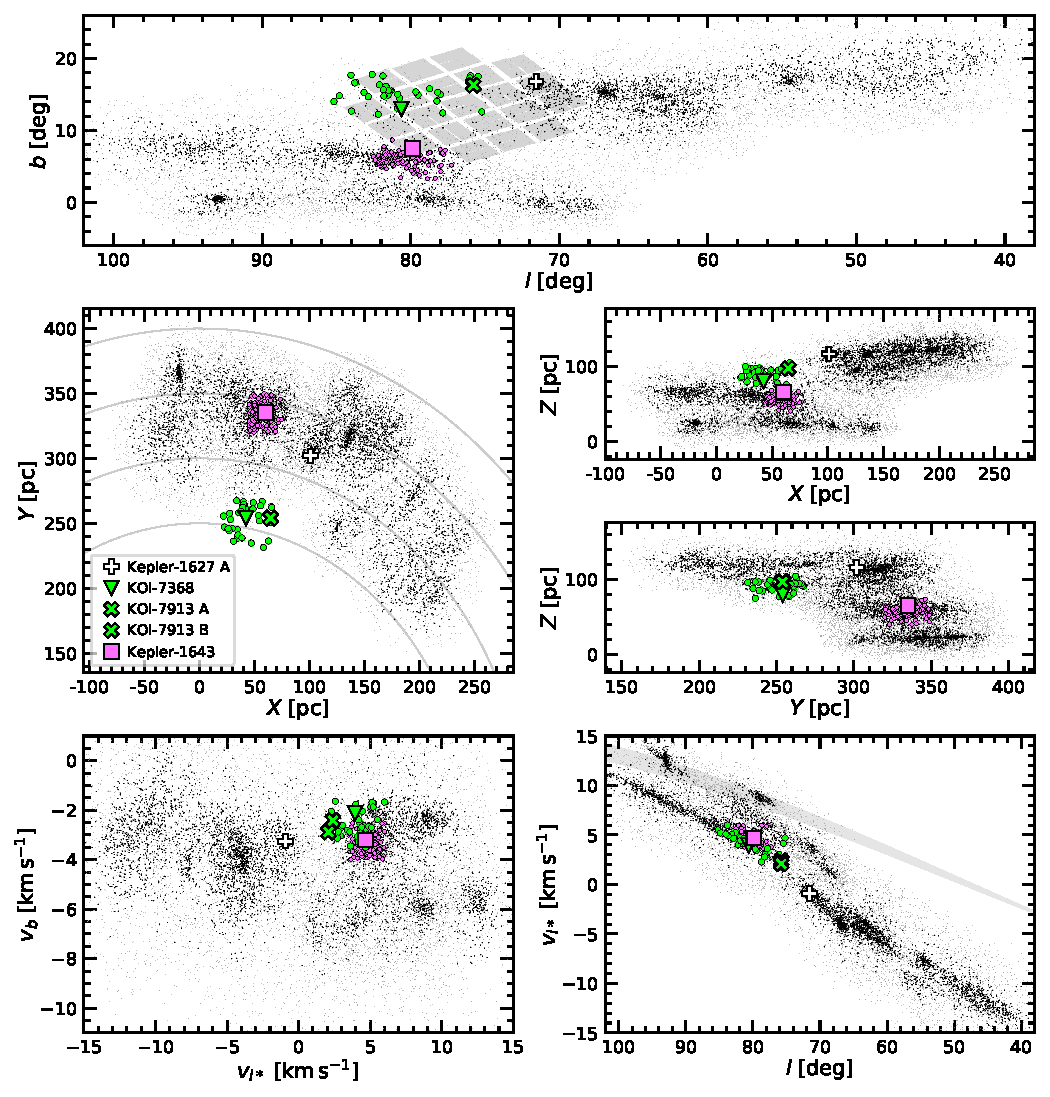
\includegraphics[width=0.99\textwidth]{f1.pdf}
	\end{center}
	\vspace{-0.7cm}
	\caption{
  {\bf Positions and velocities of candidate members of the Cep-Her
  complex.}
  {\it Top row}: On-sky positions in galactic coordinates.  Black
  points are stars for which group membership is more secure than for
  gray points.
  Kepler-1627 is in the outskirts of the $\delta$ Lyr cluster
  \citep{bouma_kep1627_2022}, which is centered at $\{ l, b\} \approx
  \{ 66^\circ, 12^\circ\}$.
  {\it Middle row}: Galactic positions.  The Sun is at $\{X, Y, Z\} =
  \{0, 0, 20.8\}$\,pc; lines of constant heliocentric distance are
  shown between 250 and 400\,pc, spaced by 50\,pc.
  {\it Bottom row}: Galactic tangential velocities (left) and
  galactic longitudinal velocity versus galactic longitude (right).
  The gray band in the lower-right shows the $\pm$1-$\sigma$
  projection of the Solar velocity with respect to the local standard
  of rest.  There is a strong spatial and kinematic overlap between
  Kepler-1643 and RSG-5 (magenta).  The local population
  of candidate young stars around KOI-7368 and KOI-7913 is more
  diffuse -- we call this region ``CH-2'' (lime-green).
  The selection method for the black, gray, purple, and green points
  is described in Section~\ref{subsec:members}.
  %The {\bf interactive figure} enables a few different cuts to be
  %shown.
	\label{fig:XYZvtang}
	}
\end{figure*}

\subsection{Previous Related Work}

Our focus is on a region of the Galaxy approximately 200 to 500\,pc
from the Sun, above the galactic plane, and spanning galactic
longitudes of roughly $40^\circ$ to $100^\circ$ degrees.  Two rich
clusters in this region are the $\delta$~Lyra cluster
\citep{stephenson_possible_1959} and RSG-5 \citep{roser_nine_2016}.
Each of these clusters was known before Gaia.  They have reported ages
between $\approx$30 and $\approx$60 million years.  Early empirical
evidence that these two clusters could be part of a large and more
diffuse population was apparent in the Gaia-based photometric analysis
of pre-main-sequence stars by \citet[][see their Figures~11
and~13]{Zari2018}.  Further kinematic connections and complexity were
highlighted by \citet{KounkelCovey2019}, who included these previously
known groups in the larger structures dubbed ``Theia~73'' and
``Theia~96''\footnote{See their visualization online at
\url{http://mkounkel.com/mw3d/mw2d.html} (accessed 15 March 2022)}.
The connection made by \citet{KounkelCovey2019} between the previously
known open clusters and the other groups in the region was made as
part of an unsupervised clustering analysis of the Gaia DR2 positions
and tangential velocities with a subsequent manual ``stitching'' step,
and generally supports the idea that there is an overdensity of
$\approx$30 and $\approx$60 million year old stars in this region of
the Galaxy.  \citet{Kerr2021}, in a volume-limited analysis of the
Gaia DR2 point-source catalog out to one third of a kiloparsec,
identified three of the nearest sub-populations, dubbed
``Cepheus-Cygnus'', ``Lyra'', and ``Cerberus''.  \citet{Kerr2021}
reported ages for each of these subgroups between 30 and 35 million
years.


\subsection{Member Selection}
\label{subsec:members}

% {\bf TODO RONAN: PLEASE VET ENTIRE SECTION, AND UPDATE WHERE
% APPROPRIATE!}.

The possibility that the $\delta$~Lyr cluster, RSG-5, and the
sub-populations identified by \citet{Kerr2021} share a common origin
has yet to be fully substantiated, and will be the subject of the upcoming
study by R.~Kerr and collaborators.  Our primary interest in the
region stems from the fact that a portion of it was observed by Kepler
(Figure~\ref{fig:XYZvtang}, top panel).  To further explore the
population of stars that were observed, we select candidate Cep-Her
members through four steps, the first three being identical to those
described in Section~3 of \citet{Kerr2021}.  We briefly summarize them
here.

The first step is to select stars that are photometrically distinct
from the field star population based on Gaia EDR3 magnitudes $\{G,
G_{\rm RP}, G_{\rm BP}\}$, parallaxes and auxiliary reddening
estimates \citep{lallement_gaia-2mass_2019}.  This step yielded \npms\
stars with high-quality photometric and astrometry, which are either
pre-main-sequence K and M dwarfs due to their long contraction
timescales, or massive stars near the zero-age main sequence due to
their rapid evolutionary timescales.

The second step is to perform an unsupervised HDBScan
clustering on the photometrically selected population
\citep{campello_hierarchical_2015,mcinnes_hdbscan_2017}.  The
parameters we use in this clustering analysis are $\{ X, Y, Z, c v_b,
c v_{l^*} \} $, where $c$ is the size-velocity corrective factor,
which is taken as $c=6\,{\rm pc / km\,s}^{-1}$ to ensure that the
spatial and velocity scales have identical standard deviations.
Positions are computed assuming the \texttt{astropy v4.0} coordinate
standard \citep{astropy_2018}, which places the Sun $8122$ pc from the
galactic center, and assumes the solar velocity with respect to the
local standard of rest from \citet{schonrich_local_2010}.  As input
parameters to HDBScan, we set the minimum $\epsilon$ threshold past
which clusters cannot be fragmented as $25$\,pc in physical space,
and $c$\,\kms\ in velocity.  The minimum cluster size $N$ is set to 10,
as is $k$, the parameter used to define the ``core distance'' density
metric. 

This unsupervised clustering in our case yielded 8 distinct groups.
These groups are then used as the ``seed'' populations for the third
step, which is to search for objects at least as close to the 10$^{\rm
th}$ nearest HDBSCAN-identified member in space-velocity coordinates.
This third step yields stars that are spatially and kinematically
close to the photometrically-young stars, but which cannot be
identified as young based on their positions in color versus absolute
magnitude.

The outcome of the analysis up to the point of the third step is shown
in Figure~\ref{fig:XYZvtang}.  To enable a selection cut that filters
out field-star contaminants, we also compute a weight metric, defined
such that the group member with the smallest core distance has a
weight of 1, the group member with the greatest core distance has a
weight of 0, and weights for the other group members are log-normally
distributed between these two extremes.  In Figure~\ref{fig:XYZvtang},
we show 12{,}436 objects with weight exceeding 0.02 as gray points,
and overplot 4{,}763 objects with weights exceeding 0.10 as black
points.\footnote{These counts only include objects with reliable astrometry
	and photometry: $\varpi/\sigma_\varpi>5$;
	$G/\sigma_{G}>50$;
	$G_{\rm RP}/\sigma_{G_{RP}}>20$;
	$G_{\rm BP}/\sigma_{G_{BP}}>20$.}
The previously known $\delta$~Lyr\ cluster ($l,b=68^\circ,15^\circ$;
$v_{l'}, v_b=-4.5 \mkms,-4 \mkms$) is visible, as is RSG-5
($l,b=83^\circ,6^\circ$; $v_{l'}, v_b=5.5 \mkms,-3.5 \mkms$).
Most of the other subclusters, including in Cep-Cyg
($l,b=90^\circ,7^\circ$) and Cerberus ($l,b=48^\circ,18^\circ$) are
too small or dispersed to have previously been analyzed in great
detail.

%
% KOI match numbers from calc_CepHer_group_numbers.py
%
The fourth and final step was to cross-match our candidate Cep-Her
member list against all known Kepler Objects of Interest.  We used the
Cumulative KOI table from the NASA Exoplanet Archive from 27 March
2022, and also compared against the \texttt{q1\_q17\_dr25} table
\citep{thompson_planetary_2018}.  From the candidate members
with weights exceeding 0.02, this yielded
 yielded 25 matches, of which 11
were known false positives, 6 were designated
``confirmed'', and 8 were designated ``candidates''.  
Inspection of the Kepler data validation summaries and Robovetter
classifications for these objects then showed whether they were
potentially consistent with being {\it i)} planets, and {\it ii)}
$\lesssim 10^8$ years old, based on the presence of rotational
modulation at the expected period and amplitude \citep[{\it
e.g.},][Figure~9]{rebull_rotation_2020}.  Four objects remained after
this inspection: Kepler-1627, Kepler-1643, KOI-7368, and KOI-7913.

Figure~\ref{fig:XYZvtang} shows the positions of the KOIs along
various projections.  Kepler-1643 is near the core RSG-5 population
both spatially and kinematically.  KOI-7368 and KOI-7913 are in a 
diffuse region $\approx$40\,pc above RSG-5 in $Z$ and $\approx$100\,pc
closer to the Sun in $Y$.  In tangential galactic velocity space,
there may be some kinematic overlap between the region the
latter two KOIs are in, and the main RSG-5 group.

%
% Numbers are from RSG-5_auto_XYZ_vl_vb_cut.csv,
% CH-2_auto_XYZ_vl_vb_cut.csv
%
We define two sets of stars in the local vicinity of our objects of
interest.  For candidate RSG-5 members, we require:
\begin{align}
  X/{\rm pc} &\in [45, 75] \nonumber \\
  Y/{\rm pc} &\in [320, 350] \nonumber \\
  Z/{\rm pc} &\in [40, 70] \nonumber \\
  v_b/{\rm km\,s^{-1}} &\in [-4, -3] \nonumber \\
  v_{l^*}/{\rm km\,s^{-1}} &\in [4, 6] \nonumber
\end{align}
For the diffuse stars near KOI-7368 and KOI-7913, we require
\begin{align}
  X/{\rm pc} &\in [20, 70] \nonumber \\
  Y/{\rm pc} &\in [230, 270] \nonumber \\
  Z/{\rm pc} &\in [75, 105] \nonumber \\
  v_b/{\rm km\,s^{-1}} &\in [-3.5, -1.5] \nonumber \\
  v_{l^*}/{\rm km\,s^{-1}} &\in [2, 6] \nonumber
\end{align}
and we call this latter set of stars ``CH-2''.  These cuts yield 141
candidate RSG-5 members, and 37 candidate CH-2 members.  An important
consideration, especially for CH-2, is the
contamination rate by field stars.  We assess this in the following
section.


\subsection{The Cluster's Age}
\label{sec:clusterage}

\begin{figure*}[tp]
	\begin{center}
		\leavevmode
		\subfloat{
			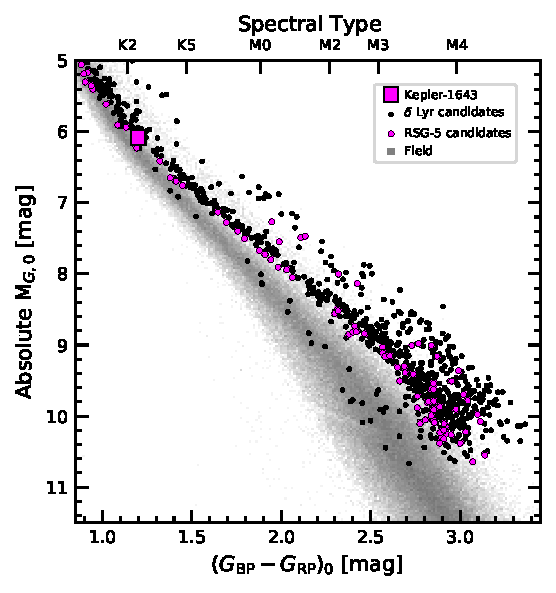
\includegraphics[width=0.49\textwidth]{f2a.pdf}
			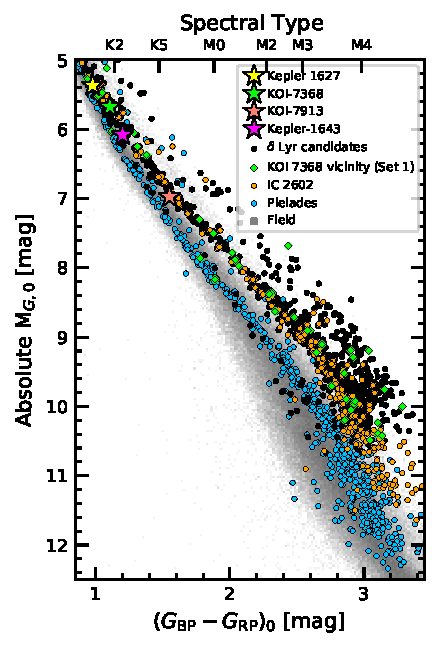
\includegraphics[width=0.49\textwidth]{f2b.pdf}
		}
		
		\vspace{-0.6cm}
		\subfloat{
			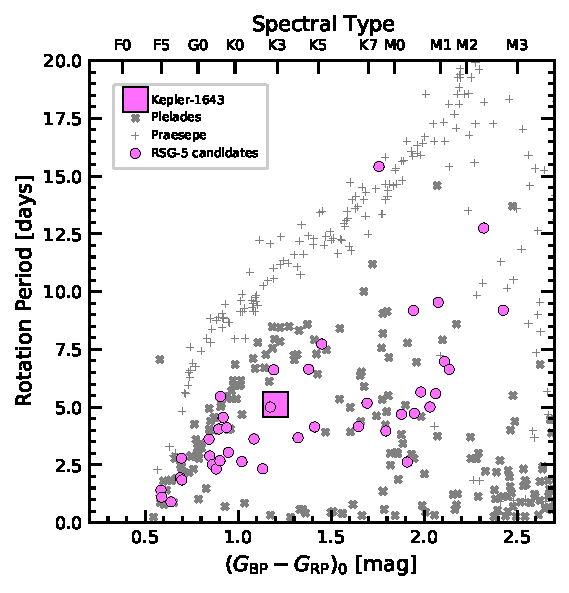
\includegraphics[width=0.49\textwidth]{f2c.pdf}
			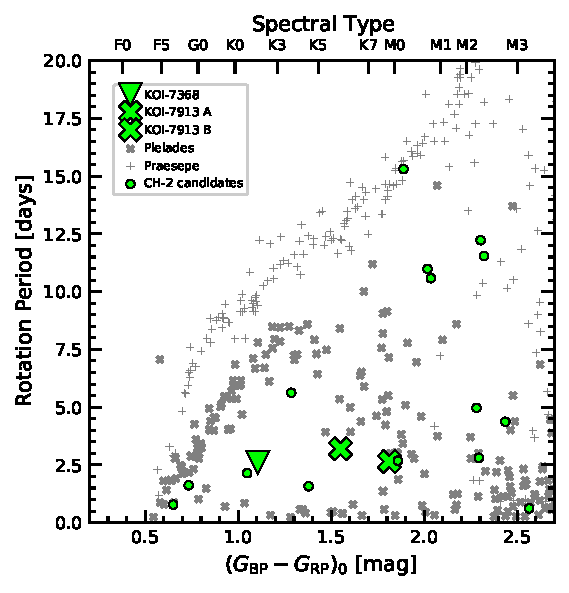
\includegraphics[width=0.49\textwidth]{f2d.pdf}
		}
	\end{center}
	\vspace{-0.7cm}
	\caption{
		{\bf The stellar groups near KOI-7368, KOI-7913, and Kepler-1643
    are 40 to 50 million years old.} 
    {\it Top row}: 
    Color-absolute magnitude diagram of candidate Cep-Her members, in
    addition to candidate members of the $\delta$~Lyr~cluster
    ($\approx38$\,Myr; \citealt{bouma_kep1627_2022}) and and the Gaia
    EDR3 Catalog of Nearby Stars (gray background).  The left and
    right columns shows stars in RSG-5 and CH-2, respectively.  The
    range of colors is truncated to emphasize the pre-main-sequence.
    {\it Bottom row}:
    TESS and ZTF-derived stellar rotation periods, with the Pleiades
    ($\approx 112$\,Myr) and Praesepe ($\approx 650$\,Myr) shown for reference
    \citep{rebull_rotation_2016a,douglas_poking_2017}.
    The detection efficiency for reliable rotation periods falls off
    beyond $\bpmrpo \gtrsim 2.6$.
	\label{fig:age}
	}
\end{figure*}

\subsubsection{Color-Absolute Magnitude Diagram}
\label{sec:camd}

Color-absolute magnitude diagrams (CAMDs) of the candidate RSG-5 and
CH-2 members are shown in the upper row of Figure~\ref{fig:age}.  The
stars from the $\delta$~Lyr cluster are from
\citet{bouma_kep1627_2022}, and the field stars are from the Gaia EDR3
Catalog of Nearby Stars \citep{gaia_gcns_2021}.  To make these
diagrams, we imposed the data filtering criteria from
\citet[][Appendix B]{GaiaCollaboration2018}, which are designed to
include binaries while omitting instrumental artifacts from for
instance low photometric signal to noise, or a small number of
visibility periods.  We then corrected for extinction using the
\citet{lallement_threedimensional_2018}\footnote{\url{https://stilism.obspm.fr/}}
dust maps and the extinction coefficients $k_X\equiv A_X/A_0$ from
\citet{GaiaCollaboration2018}, assuming that $A_0 = 3.1 E(B-V)$.  This
yielded a mean and standard deviation for the reddening of
$E(B-V)=0.036\pm0.002$ for RSG-5, and $E(B-V)=0.017\pm0.001$
for CH-2.  By way of comparison, in \citet{bouma_kep1627_2022} the
same query for the $\delta$~Lyr cluster yielded
$E(B-V)=0.032\pm0.006$.  Finally, for the plots we set the $\bpmrpo$
color range to best visualize the region of maximal age information
content: the pre-main-sequence.

The CAMDs show that for RSG-5, our membership selection gives stars
that photometrically seem to almost all be on a tight
pre-main-sequence locus.  This implies a false positive rate of 
a few percent, at most.  By comparison, our control sample (the $\delta$~Lyr
candidates) has a false positive rate of $\approx$12\%, based on the
number of stars that photometrically appear to be more consistent with
the field population than the bulk cluster population.  For CH-2, our
membership selection gives 27 objects in the color range displayed,
and 23 of them appear to be consistent with being on the
pre-main-sequence.  This implies a false positive rate of
$\approx$15\%.

In addition, Figure~\ref{fig:age} shows that the candidate RSG-5 and
CH-2 members overlap with the $\delta$~Lyr cluster, and are therefore
roughly the same age.  To quantify this, we use the empirical method
introduced by \citet[][see their Section~6.3]{gagne_mutau_2020}.  This
idea of the method is to fit the pre-main-sequence loci of a set of
reference clusters, and to then model the locus of the target cluster
as a linear combination of these reference cluster loci.  For our
reference clusters, we used UCL, IC\,2602, and the Pleiades, from the
memberships reported by \citet{Damiani2019} and
\cite{CantatGaudin2018a} respectively.  We adopted ages of 16\,Myr for
UCL \citep{pecaut_star_2016}, 38\,Myr for IC\,2602\footnote{ Ages for
IC\,2602 vary from 40 to 46\,Myr based on lithium-depletion-boundary
(LDB) measurements \citep{dobbie_ic_2010,randich_gaiaeso_2018}, and
from 30 to 46\,Myr based on isochronal analyses
\citep{stauffer_rotational_1997,david_ages_2015,bossini_age_2019}.},
and 112\,Myr for the Pleiades \citep{dahm_2015}.  These assumptions
and the consequent processing steps taken to exclude field stars as
well as photometric and astrometric binaries were identical to those
described in \citet{bouma_kep1627_2022}.  The mean and standard
deviation of the resulting age posterior are $46^{+9}_{-7}$\,Myr for
RSG-5, and $36^{+10}_{-8}$\,Myr for CH-2.  For comparison, the this
procedure yields an age for the $\delta$~Lyr cluster of
$38^{+6}_{-5}$\,Myr.  The slightly older isochronal age of RSG-5 is
expected given that its locus is slightly bluer and less luminous in
the upper left panel of Figure~\ref{fig:age} relative to the
$\delta$~Lyr cluster.


\subsubsection{Stellar Rotation Periods}
\label{sec:rotation}

An independent way to assess the age of the candidate cluster members
is to measure their stellar rotation periods.  This approach can be
achieved using surveys such as TESS \citep{ricker_transiting_2015} and
ZTF \citep{bellm_zwicky_2019}, and it leverages a storied tradition of
rotation period measurement for benchmark open clusters \citep[see
{\it e.g.},][]{skumanich_time_1972,curtis_rup147_2020}.  The TESS data
in our case are especially useful, since they provide 3 to 5 lunar
months of photometry for all of our candidate CH-2 and RSG-5 members.

We selected stars suitable for gyrochronology by requiring $\bpmrpo
\geq 0.5$ and $G<16$.  The latter cut corresponds to $\bpmrpo \lesssim
2.6$, at the relevant distances.  These cuts gave 19 stars in CH-2 and
42 stars in RSG-5.  We extracted light curves from the TESS images for
these stars using the \texttt{unpopular} package
\citep{hattorio_2021_cpm}, and regressed them against systematics with
its causal pixel model.  {\bf For the ZTF light curves, we used the
default photometry?  Ran aperture photometry on the image cutouts?}.
We then measured candidate rotation periods using a Lomb-Scargle
periodogram, and visually inspected them following the methods
discussed in \citet{curtis_rup147_2020}.

The lower panels of Figure~\ref{fig:age} show the results.  In RSG-5,
36/42 stars have rotation periods faster than the Pleiades (86\%).
This numerator omits the two stars with periods $>12$\,days visible in
the lower-left panel of Figure~\ref{fig:age}.  The age interpretation
for these latter stars, particularly the $\approx$M2.5 dwarf, is not
obvious.  \citet{rebull_usco_2018} for instance have found numerous
M-dwarfs with 10-12 day rotation periods at ages of USco ($\sim
8$\,Myr), and some may still exist at ages of LCC ($\sim 16$\,Myr;
L.~Rebull in preparation).  Regardless, given that nearly no field
star outliers seem to be present on the RSG-5 CAMD, the fact that we
do not detect rotation periods for $\approx$14\% of stars should
perhaps be taken as an indication for the fraction of stars for
rotation periods might not be detectable, due to {\it e.g.}, pole-on
stars having lower amplitude starspot modulation.

%
% CH-2
% 5 stars with Prot>10 days (from the Prot versus color plot):
%                      DESIGNATION  TESS_Data   bp_rp_x     period
%25  Gaia EDR3 2129930258400157440          4  1.909693  15.309000
%24  Gaia EDR3 2129417404945830784          4  2.040988  10.981582
%4   Gaia EDR3 2107169165113864064          4  2.059904  10.580494
%9   Gaia EDR3 2134851775526125696          4  2.326998  12.227900
%1   Gaia EDR3 2127726081184588160          4  2.347244  11.543281
%
% CH-2
% Photometric field stars (from Glue -- one of these is omitted due to phot S/N cut, 
% presumably 2126008609657702784 )
%
%In [9]: df[['DESIGNATION', 'bp_rp', 'M_G']]
%Out[9]:
%                     DESIGNATION     bp_rp        M_G
%0  Gaia EDR3 2126529468937923456  2.518077   9.844733 --> NaN period, G=16.9
%1  Gaia EDR3 2126008609657702784  2.746735  11.409737 --> NaN, G=18.4
%2  Gaia EDR3 2133330051428541952  2.499458   9.459546 --> 15.7 d (ZTF), G=16.5
%3  Gaia EDR3 2133510921093964928  2.720177  10.923209 --> NaN, G=17.9
%4  Gaia EDR3 2139369183468814464  2.929506  11.170221 --> NaN, G=18.2
%5  Gaia EDR3 2129930258400157440  1.909693   8.200652 --> P=15.3 (ZTF), G=15.2

For CH-2, 13/19 stars have rotation periods that are obviously faster
than their counterparts in the Pleiades (68\%).  4 stars, not included
in the preceding numerator, are M-dwarfs with rotation periods between
10 and 12.5 days.  The age interpretation for these M-dwarfs is, as
just discussed, not obvious.  Regardless, the $\approx$15\% false
positive rate determined from the CAMD seems consistent with our
fraction of detected rotation periods, given that RSG-5 was also
missing rotation period detections for $\approx$15\% of its candidate
members, which all seemed photometrically consistent with being part
of a single pre-main-sequence locus.

It is challenging to convert these stellar rotation periods
to a precise age estimate, since on the pre-main-sequence
the stars are spinning up due to thermal contraction
rather than down due to magnetized braking.  Regardless, the rotation
period distributions of both CH-2 and RSG-5 seem consistent with other
30\,Myr to 50\,Myr clusters ({\it e.g.}, IC\,2602 and IC\,2391;
\citealt{douglas_stephanie_t_2021_5131306}).
They also seem consistent with the false positive rate estimates
determined from the color-absolute magnitude diagrams.


\section{The Stars}
\label{sec:stars}

\begin{deluxetable}{lccc}
\tabletypesize{\scriptsize}
\tablecaption{Selected system parameters of Kepler-1643, KOI-7368, and KOI-7913. \label{tab:sysparams}}
\tablenum{1}

\tablehead{
\colhead{Parameter} & \colhead{Value} & \colhead{68\% Confidence Interval} & \colhead{Comment}
}

\startdata
\hline
\multicolumn{4}{c}{\emph{Kepler-1643}} \\
\hline
{\it Stellar parameters:} & & & \\
  Gaia $G$~[mag]                             & $13.836$           & $\pm 0.003$                & A \\
  $T_{\rm eff}$~[K]                          & $4916$             & $\pm 110$                  & B \\
  %$\log g_\star$~[cgs]                      & $4.54$             & $\pm 0.10$                 & D \\
  $\log g_\star$~[cgs]                       & $4.502$            & $\pm 0.035$                & C \\
  $R_\star$~[R$_{\odot}$]                    & $0.855$            & $\pm 0.044$                & C \\
  $M_\star$~[M$_{\odot}$]                    & $0.845$            & $\pm 0.025$                & C \\
  $\rho_\star$~[g~cm$^{-3}$]                 & $1.910$            & $\pm 0.271$                & C \\
  $P_{\rm rot}$~[days]                       & $5.106$            & $\pm 0.044$                & D \\
  Li EW~[m\AA]                               & $126$              & $+8$, $-4$                 & E \\
{\it Transit parameters:} & & & \\
%  $t_0$~[BJD$_{\rm TDB}$]                   & $X$                & $X$                        & D \\
  $P$~[days]                                 & $X$                & $X$                        & D \\
  $R_{\rm p}/R_\star$                        & $0.X$              & $+0.X$, $-0.X$             & D \\
  $b$                                        & $X$                & $X$                        & D \\
%  $a/R_\star$                               & $X$                & $+0.X$, $-0.X$             & D \\
  $R_{\rm p}$~[R$_{\oplus}$]                 & $X$                & $\pm 0.X$                  & D \\
  $t_{14}$~[hours]                           & $X$                & $X$                        & D \\
\hline
\multicolumn{4}{c}{\emph{KOI-7368}} \\
\hline
{\it Stellar parameters:} & & & \\
  Gaia $G$~[mag]                             & $12.831$           & $\pm 0.004$                & A \\
  $T_{\rm eff}$~[K]                          & $5241$             & $\pm 50$                   & F \\
  $\log g_\star$~[cgs]                       & $4.499$            & $\pm 0.030$                & C \\
  $R_\star$~[R$_{\odot}$]                    & $0.876$            & $\pm 0.035$                & C \\
  $M_\star$~[M$_{\odot}$]                    & $0.879$            & $\pm 0.018$                & C \\
  $\rho_\star$~[g~cm$^{-3}$]                 & $1.840$            & $0.225$                    & C \\
  $P_{\rm rot}$~[days]                       & $2.606$            & $0.038$                    & D \\
  Li EW~[m\AA]                               & $X$                & $X$                        & B \\
{\it Transit parameters:} & & & \\
 % $t_0$~[BJD$_{\rm TDB}$]                    & $X$                & $X$                        & D \\
  $P$~[days]                                 & $X$                & $X$                        & D \\
  $R_{\rm p}/R_\star$                        & $0.X$              & $+0.X$, $-0.X$             & D \\
  $b$                                        & $X$                & $X$                        & D \\
%  $a/R_\star$                                & $X$                & $+0.X$, $-0.X$             & D \\
  $R_{\rm p}$~[R$_{\oplus}$]                 & $X$                & $\pm 0.X$                  & D \\
  $t_{14}$~[hours]                           & $X$                & $X$                        & D \\
\hline
\multicolumn{4}{c}{\emph{KOI-7913 A}} \\
\hline
{\it Stellar parameters:} & & & \\
  Gaia $G$~[mag]                             & $14.200$           & $\pm 0.003$                & A \\
  $T_{\rm eff}$~[K]                          & $4324$             & $\pm 70$                   & B \\
  $\log g_\star$~[cgs]                       & $4.523$            & $\pm 0.043$                & C \\
  $R_\star$~[R$_{\odot}$]                    & $0.790$            & $\pm 0.049$                & C \\
  $M_\star$~[M$_{\odot}$]                    & $0.760$            & $\pm 0.025$                & C \\
  $\rho_\star$~[g~cm$^{-3}$]                 & $2.172$            & $\pm 0.379$                & C \\
  $P_{\rm rot}$~[days]                       & $3.387$            & $0.016$                    & D \\
  Li EW~[m\AA]                               & $X$                & $X$                        & B \\
  $\Delta G_{\rm AB}$~[mag]                  & $0.51$             & $0.01$                     & F \\
  Apparent sep.~[au]                   		   & $959.4$            & $1.9$                      & F \\
{\it Transit parameters:} & & & \\
  %$t_0$~[BJD$_{\rm TDB}$]                    & $X$                & $X$                        & D \\
  $P$~[days]                                 & $X$                & $X$                        & D \\
  $R_{\rm p}/R_\star$                        & $0.X$              & $+0.X$, $-0.X$             & D \\
  $b$                                        & $X$                & $X$                        & D \\
%  $a/R_\star$                                & $X$                & $+0.X$, $-0.X$             & D \\
  $R_{\rm p}$~[R$_{\oplus}$]              & $X$                & $\pm 0.X$                  & D \\
  $t_{14}$~[hours]                           & $X$                & $X$                        & D \\
\enddata
\tablecomments{
  (A) \citet{gaia_collaboration_2021_edr3}.
  (B) HIRES SpecMatch-Emp \citep{yee_SM_2017}.
  (C) Cluster isochrone \citep{choi_mesa_2016, bressan_parsec_2012}.
  (D) Kepler light curve.  The full set of transit parameters is given in CITE APPENDIX TABLE.
  (E) HIRES; this work.
  (F) TRES SPC \citep{buchhave_hatp16b_class_2010,2021tsc2.confE.124B}.
  (G) Magnitude difference and physical distance between primary and secondary; from Gaia EDR3.
  (H) HIRES SpecMatch-Synth \citep{petigura_cksi_2017}.
}
%\vspace{-1cm}
\end{deluxetable}


Some salient stellar parameters of the KOIs in Cep-Her can be gleaned
by inspecting Figure~\ref{fig:age}.  They span spectral types of G8V
(Kepler-1627) to K8V (KOI-7913 A).  The secondary in the KOI-7913
system is only marginally cooler than the primary.  And since a
Solar-mass star with solar metallicity arrives at the zero-age main
sequence at $t\approx40$ million years \citep{choi_mesa_2016}, these
stars are all in the late stages of their pre-main-sequence
contraction.  Their heliocentric distances are $\approx$260\,pc
(KOI-7913 and KOI-7368, in CH-2) and $\approx$340\,pc (Kepler-1643, in
RSG-5).

The adopted stellar parameters are listed in
Table~\ref{tab:sysparams}.  The stellar surface gravity, radius,
mass, and density are found by interpolating against the MIST
isochrones \citep{choi_mesa_2016}.  The statistical uncertainties from
this technique mostly originate from the parallax uncertaintes; the
systematic uncertainties are taken to be the absolute difference
between the PARSEC \citep{bressan_parsec_2012} and MIST isochrones.
Reported uncertainties are a quadrature sum of the statistical and
systematic components. 

To verify these parameters and to also analyze spectroscopic youth
proxies such as the Li\,\textsc{I} 6708\,\AA\ doublet and H$\alpha$,
we acquired spectra.  We also acquired high resolution imaging for
each system, to constrain the existence of visual companions,
including possible bound binaries.  The system-by-system details
follow, and the the relevant results are also summarized in
Table~\ref{tab:sysparams}.

\subsection{Kepler\,1643}

\paragraph{Spectra}
For Kepler-1643, we acquired two iodine-free spectra from Keck/HIRES
on the nights of 2020 August 16 and 2021 October 25.  The acquisition
and analysis followed the standard reduction techniques of the
California Planet Survey \citep{howard_cps_2010}.  We derived the
stellar parameters ($T_{\rm eff}, \log g, R_\star$) using
\texttt{SpecMatch-Emp} \citep{yee_SM_2017}, which yielded values in
$<1$-$\sigma$ agreement with those from the cluster-isochrone
approach.  This approach also yielded $[{\rm Fe/H}]=0.13 \pm 0.09$.
Using the broadened synthetic templates from \texttt{SpecMatch-Synth}
\citep{petigura_cksi_2017}, we found $v\sin i = 9.3 \pm 1.0\,\mkms$.
The systemic radial velocity at the two sequence epochs was $-9.1 \pm
1.9\,\mkms$ and $-7.8\pm 1.2\,\mkms$ respectively.  To infer the
equivalent width of the Li\,\textsc{I} 6708\,\AA\ doublet, we followed
the procedure described by \citet{bouma_2021_ngc2516}.  This yielded a
strong detection: ${\rm EW}_{\rm Li} = 126^{+8}_{-4}$\,m\AA, with
values consistent at $<1$-$\sigma$ between the two epochs.   The
quoted value does not correct for the Fe\,\textsc{I} blend at
6707.44\AA.  

% {\bf TODO verify continuum normalization in Li EW measurement...}
% Given the reddening-corrected color of the star this is
% consistent(ish) with the Pleiades/NGC2516 based on my NGC2516 figure.
% But it looks sub-IC2602 based on the lithium.png figure, which uses
% the Randich2018 values.
% It's pretty clearly super-field.
% I really need to verify the continuum normalization.
% COMPARE vs:
% \citealt{randich_gaiaeso_2018}).  
% \citet{berger_identifying_2018}

\paragraph{High-Resolution Imaging}
% KOI-6186 & 58662.62 &   Kp     &  4 &   80.00 &  4.1 &  4.8 &  5.4 &  5.8 &  6.5 &  6.8 &  7.6 &  8.3 &  8.2 &  8.3 &             Petigura \\ % N2.20190628.53389
We acquired adaptive optics imaging of Kepler-1643 on the night of
2019 June 28 using the NIRC2 imager on Keck-II (PI: E.~Petigura).
Using the narrow camera (FOV = 10.2\arcsec), we obtained 4 images in
the $K'$ filter ($\lambda = 2.12\,\mu$m) with a total exposure time of
320\,s. We analyzed these data following \citet{kraus_impact_2016},
and determined the detection limits to visual companions by analyzing
the residuals after subtracting an empirical PSF template. 
This procedure yielded contrast limits of $\Delta K' = 4.1$ mag at
$\rho = 150$ mas, $\Delta K' = 5.8$ mag at $\rho = 300$ mas, and
$\Delta K' = 8.3$ mag at $\rho > 1000$ mas.


\subsection{KOI-7368}
\paragraph{Spectra}
For KOI-7368, we acquired a spectrum on 2015 June 1 using the echelle
spectrograph (TRES; \citealt{furesz_tres_2008}) mounted at the
Tillinghast 1.5m at the Fred Lawrence Whipple Observatory on Mt.
Hopkins, AZ.  The stellar parameter classification pipeline for the
TRES spectra has been described by \citet{2021tsc2.confE.124B}.  It is
based on the synthetic template library originally constructed by
\citet{buchhave_hatp16b_class_2010}.  The resulting stellar parameters
($T_{\rm eff}, \log g, R_\star$) agreed with those from the
cluster-isochrone method within $1$-$\sigma$, though the effective
temperature is more precise by a factor of three.  Auxiliary
spectroscopic parameters included the metallicity $[{\rm Fe/H}]= -0.02
\pm 0.08$, the equatorial velocity $v\sin i = 20.21 \pm 0.50\,\mkms$,
and the systemic velocity ${\rm RV}_{\rm sys} = -10.9 \pm 0.2\,\mkms$.
The Li 6708\AA\ EW measurement procedure yielded ${\rm EW}_{\rm Li} =
236^{+16}_{-14}$\,m\AA.

\paragraph{High-Resolution Imaging}
% KOI-7368 & 58646.57 &   Kp     &  4 &   80.00 &  5.2 &  5.8 &  6.4 &  6.7 &  7.1 &  7.5 &  8.1 &  8.7 &  8.7 &  8.8 &                Huber \\ % N2.20190612.49290
We acquired adaptive optics imaging of KOI-7368 on the night of 2019
June 12 using the NIRC2 imager on Keck-II (PI: D.~Huber).  The
observational configuration and reduction was identical as for
Kepler-1643.  No companions were detected, and the analysis of the
image residuals yielded contrast limits of $\Delta K' = 5.2$ mag at
$\rho = 150$ mas, $\Delta K' = 6.7$ mag at $\rho = 300$ mas, and
$\Delta K' = 8.7$ mag at $\rho > 1000$ mas.


\subsection{KOI-7913}

\paragraph{Binarity}

%(e.g., Jenkins KSCI-19081-002 KPDH pp 129, or many other pages)
KOI-7913 is almost certainly a binary.\footnote{Relevant identifiers for the
primary are KIC 8873450 = Gaia DR2/EDR3 2106235301785454208.  For the
secondary, they are KIC 8873448 = Gaia DR2/EDR3 2106235301785453824.}
The north-west primary is $\approx$0.5 magnitudes brighter than the
south-east secondary in optical passbands.  The two stars are
separated in Gaia EDR3 by $3\farcs54$ on-sky, and have parallaxes
consistent within $1$-$\sigma$ (with an average $\varpi=3.66 \pm
0.01$\,mas).  This corresponds to an apparent on-sky separation of
$959 \pm 2$ au.  Gaia EDR3 quotes
$(\mu_{\alpha'},\mu_\delta)=(2.439\pm0.015, 1.009\pm 0.016)\,{\rm
mas}\,{\rm yr}^{-1}$ for the primary, and
$(\mu_{\alpha'},\mu_\delta)=(2.696\pm0.020, 0.650 \pm 0.021) \,{\rm
mas}\,{\rm yr}^{-1}$ for the secondary.  Since two stars were resolved
in the Kepler Input Catalog and are roughly one Kepler pixel apart, an
accurate crowding metric has already been applied in the NASA Ames
data products to correct the mean flux level
\citep{2017ksci.rept....6M}.  This is important for deriving accurate
transit depths.

\paragraph{Spectra}

We acquired Keck/HIRES spectra for KOI-7913 A on the night of 2021 Nov
13, and KOI-7913 B on the night of 2021 Oct 26.  The usual
\texttt{SpecMatch-Emp} \citep{yee_SM_2017} machinery yielded $T_{\rm
eff,A} = 4324 \pm 70\,{\rm K}$, $T_{\rm eff,B} = 4038 \pm 70\,{\rm
K}$.  The remaining parameters were in agreement with those from the
cluster isochrone.  For the primary, we also found $[{\rm Fe/H}]=
-0.06 \pm 0.09$, $v\sin i = 13.3 \pm 1.0\,\mkms$, and ${\rm RV}_{\rm
sys} = -17.8 \pm 1.1\,\mkms$.  These same parameters for the secondary
were $[{\rm Fe/H}]= -0.01 \pm 0.09$, $v\sin i = 10.7 \pm 1.0\,\mkms$,
and ${\rm RV}_{\rm sys} = -18.8 \pm 1.1\,\mkms$.

Regarding indicators of youth, the primary has a spectral type
$\approx$K6V, while the secondary is $\approx$M0V.  At $\approx$40
Myr, lithium 6708\,\AA\ absorption is not expected for the secondary,
but might be present in the primary \citep[{\it
e.g.},][Figure~8]{soderblom_ages_2014}.  Conversely, H$\alpha$ is
expected to be in emission for for all M-dwarfs younger than
$\approx150$\,Myr \citep{kiman_calibration_2021}.  At $\approx$M0V, if
the secondary were in older than $\approx 500\,{\rm Myr}$, it would be
more common for its H$\alpha$ component to be observed in absorption
\citep[][Figure~4]{kiman_calibration_2021}.  H$\alpha$ emission in
late K-dwarfs is rarer still. Based on the data from K.~Rocio et al's
analysis\footnote{Available at
\url{https://zenodo.org/record/4659293\#.YkuKh27MKDV}}, a $\approx$K6V
star should be emitting in H$\alpha$ at 40\,Myr, but not typically
past $\approx200\,{\rm Myr}$.  This presents a fairly direct test for
the star's age.

Turning to the actual data, we find {\bf X for lithium}.
For H$\alpha$, {\bf we see Y}.

% For Li:
%    ~~~(CITE Figure 10 of Barrado y Navasceus 2004?).
%   ****USE FIG8 OF SODERBLOM+13****
% 
%   OR USE BAFFLES AS YOUR REFERENCE?
%     B-V=1.48 (primary), IC2602 age has no data.  beta pic age has lots of scatter
%     around this color, between 10mA and 100mA.
%     B-V=redder... 1.8?  SpType ~M0V, really no Li expected.
%   A: no... they really didn't collect very good data from what i see.
%   especially at the red end...
% 
% NW component SpType~K5.5-K6V; HIRES spectrum shows weak Li (EW 65 +/-
% 8 mA), Halpha in emission (double-peaked?!), and CaHK in emission.
% Reamatch SB2 checks don't show evidence for it being SB2.
% SW component SpType~K9V-M0V; HIRES spectrum shows H-alpha in emission
% (consistent with <150 Myr) and no Li (expected given Teff).
% Given the kinematics, the spectra paint a picture consistent with KOI
% 7913 being part of the ~40 Myr Cep-Her group.

\paragraph{High-Resolution Imaging}

We acquired adaptive optics imaging of KOI-7913 on the night of 2020
Aug 27 using the NIRC2 imager on Keck-II (PI: D.~Huber).  The
observational configuration and reduction was identical as before.
The images showed KOI-7913 A, KOI-7913 B, and an additional faint star
$\approx0\farcs99$ due East of KOI-7913 B.  Applying the PSF-fitting
routines from \citet{kraus_impact_2016}, the tertiary star has a
separation $\rho = 4397 \pm 3$\,mas from the primary, at a position
angle $231.17^\circ \pm 0.02^\circ$, with a $\Delta K' = 6.97 \pm
0.04$.  While it is too faint to affect the interpretation of the KOI
itself, it would be amusing if the faint neighbor were also comoving
and young -- at the age of the system, it would have a mass roughly
between 10 and 15\,M$_{\rm Jup}$.  Additional imaging epochs will be
required to tell.




\section{The Planets}
\label{sec:planets}

\begin{figure*}[tp]
	\begin{center}
		\leavevmode
		\subfloat{
			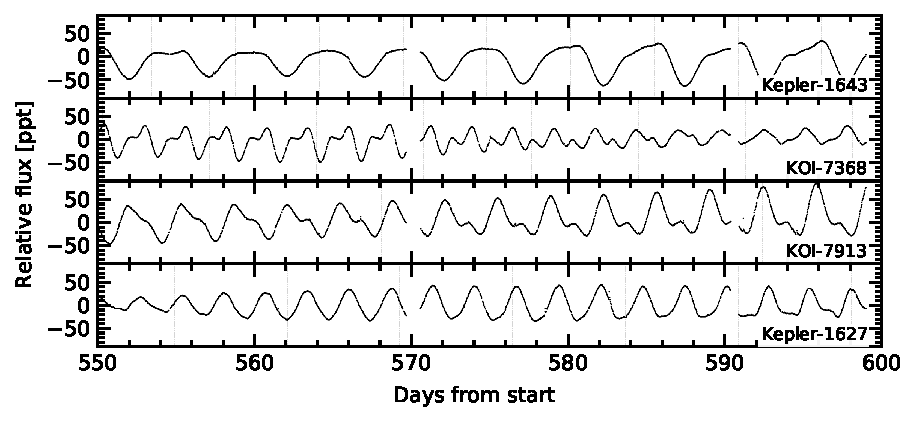
\includegraphics[width=0.85\textwidth]{f3e.pdf}
		}

		\vspace{-0.5cm}
		\subfloat{
			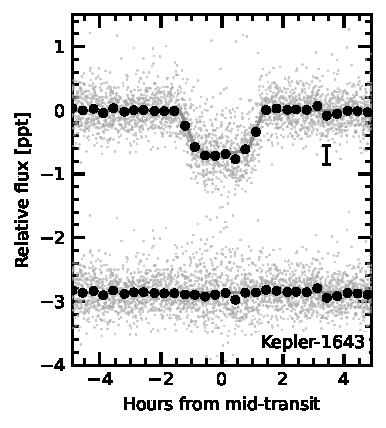
\includegraphics[width=0.33\textwidth]{f3a.pdf}
			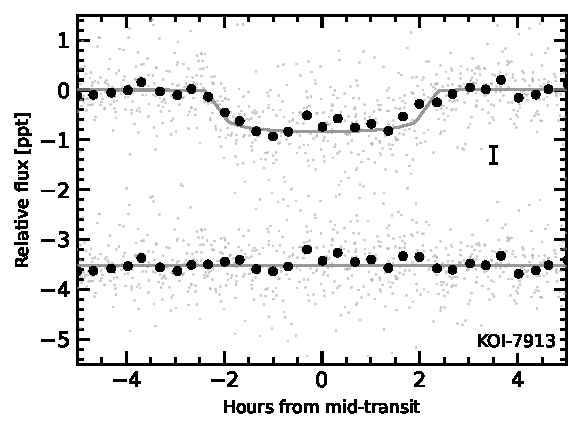
\includegraphics[width=0.33\textwidth]{f3b.pdf}
		}

		\vspace{-1.27cm}	
		\subfloat{
			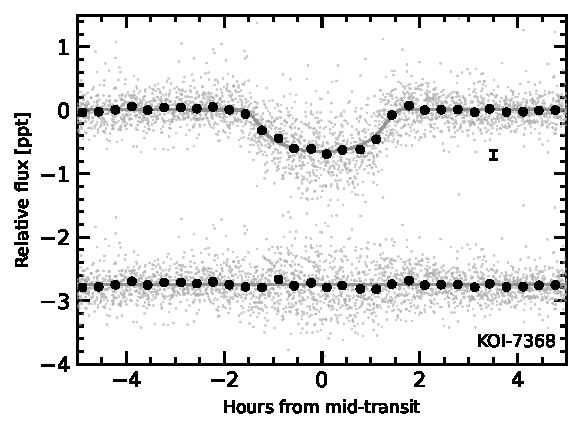
\includegraphics[width=0.33\textwidth]{f3c.pdf}
			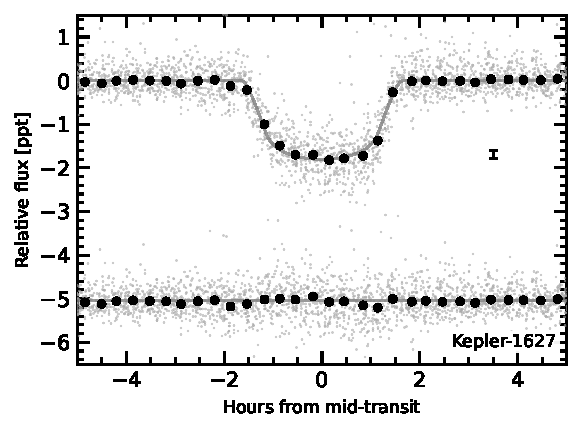
\includegraphics[width=0.33\textwidth]{f3d.pdf}
		}
	\end{center}
	\vspace{-0.5cm}
	\caption{
		{\bf Raw and processed light curves for the Kepler Objects of
    Interest in Cep-Her.}   
    {\it Top}:
    50 day light curve segment from the 3.9 years of Kepler data.  The
    ordinate shows the \texttt{PDCSAP} median-subtracted flux in units
    of parts-per-thousand ($\times 10^{-3}$).  The dominant signal is
    induced by starspots.  
    {\it Bottom}:
    Phase-folded transits of Kepler-1643, KOI-7913, KOI-7368, and
    Kepler-1627 with stellar variability removed.  The maximum {\it a
    posteriori} transit model is shown with the gray line, and the
    residual after subtracting the transit model is vertially
    displaced.  Windows over 10 hours are shown.  Gray points are
    individual flux measurements; black points are binned to 20 minute
    intervals, and have a representative 1-$\sigma$ error bar in the
    center-right of each panel. 
		\label{fig:planets}
	}
\end{figure*}

\subsection{Kepler Data}

The Kepler space telescope observed Kepler-1643, KOI-7913, and
KOI-7368 at a 30-minute cadence between May 2009 and April 2013.  For
all three systems quarters 1 through 17 were observed without any data
gaps other than the usual quarterly roll.  The top panel of
Figure~\ref{fig:planets} shows a 50-day slice of the \texttt{PDCSAP}
light curves for the three new Cep-Her candidates, along with
Kepler-1627.  In \texttt{PDCSAP}, nonastrophysical variability is
removed through a cotrending approach that uses a set of basis vectors
derived using singular value decomposition of a set of
systematics-dominated stellar light curves
\citep{smith_kepler_PDC_2017}.  In our analysis, we used the
\texttt{PDCSAP} light curves with the default optimal aperture
\citep{smith_finding_2016}.  Cadences with non-zero quality flags were
omitted.  In all cases, the stars are dominated by spot-induced
modulation with peak-to-peak variability between 2\% and 10\%.  These
signals are much larger than the transits, which have depth
$\approx$0.1\%.
To quantify the stellar rotation periods, we calculated the
Lomb-Scargle periodogram for each Kepler quarter independently.  The
resulting means and standard deviations are quoted in
Table~\ref{tab:sysparams}.


\subsection{Transit and Stellar Variability Model}
\label{sec:fitting}

Our goals in fitting the Kepler light curves are twofold.  First, we
want to derive accurate planetary sizes and orbital properties.
Second, we want to remove the stellar variability signal to enable a
statistical assessment of the probability that the transit signals are
planetary.

Our adopted approach was as follows.  Given an initial guess for the
transit ephemeris from the \texttt{q1\_q17\_dr25} analysis
\citep{thompson_planetary_2018}, the light curve was first trimmed to
a local window around each transit of duration $\pm 3\times t_{14}$.
The local out-of-transit points were then fitted with a fourth-order
polynomial, which was then divided out from the light curve.  The
resulting flattened transits were then fitted with a 
planetary transit under the assumption of quadratic limb darkening.
Our model therefore included 8 free parameters for the transit ($\{P,
t_0, \log R_{\rm p}/R_\star, b, u_1 ,u_2, R_\star, \log g\}$), 2 free
parameters for the light curve normalization and a white noise jitter
($\{\langle f \rangle, \sigma_f \}$), and an additional 5 implicit
parameters per transit through the polynomial.

We fitted the models using \texttt{exoplanet}
\citep{exoplanet:exoplanet}.  We assumed a Gaussian likelihood, and
sampled using \texttt{PyMC3}'s No-U-Turn Sampler
\citep{hoffman_no-u-turn_2014}, after having initialized using the
maximum {\it a posteriori} (MAP) model.  We used the
\citet{gelman_inference_1992} statistic ($\hat{R}$) as our convergence
diagnostic.  The results are shown in the lower panels of
Figure~\ref{fig:planets}, and the important derived parameters are in
Table~\ref{tab:sysparams}.  The set of full parameters with their
priors are given in Appendix~\ref{app:transit}.

One weakness of our fitting approach is that we have fixed 5 implicit
parameters per individual transit to their MAP values to remove the
stellar variability signal.  An alternative could be to fit the
planetary transits simultaneously with the starspot-induced
variability using, say, a quasiperiodic Gaussian process (GP).  We
explored this approach, but found that it required careful fine-tuning
of the hyperparameter priors, otherwise the GP would tend to
incorporate any variability that was not part of the transit, even if it was
short-term variability attributable to flares, or simply
instrumental noise.  This failure mode is somewhat pernicious, in that
it yields an ill-founded sense of confidence in an ``overly clean''
transit model fit.  Although our model is simpler, it has the benefit
that the white noise jitter never trades off with any parameter
equivalent to a damping timescale for the coherence of the GP.  It is
also computationally efficient, and it captures the planetary
parameters that we actually care about.


\subsection{Planet Validation}

In the future, it may be possible to obtain independent evidence for
the Cep-Her planets to directly confirm their planetary nature.  The
most likely path would be through transit observations using a
high-resolution spectrograph \citep[see][]{bouma_kep1627_2022}.  In
the interim, it is of interest whether the transit signals could be
astrophysical false positives, or whether they can be argued to be
planetary on a statistical basis.  We adopt the Bayesian framework
implemented in \texttt{VESPA} for this purpose
\citep{morton_efficient_2012,vespa_2015}.  Briefly summarized, the
priors in \texttt{VESPA} take as given the binary star occurrence rate
from \citet{raghavan_survey_2010}, direction-specific star counts from
\citet{girardi_star_2005}, and planet occurrence rates as described by
\citet[][Section~3.4]{morton_efficient_2012}.  The likelihoods are
then evaluated by forward-modeling a synthetic population of eclipsing
bodies for each possible astrophysical model class, in which each
population member has a particular trapezoidal eclipse depth, total
duration, and ingress duration.  These summary statistics are then
compared against the actual photometric data to evaluate the
probabilities of false positive scenarios such as foreground eclipsing
binaries, hierarchical eclipsing binaries, and background eclipsing
binaries.

\paragraph{Kepler-1643}
Kepler-1643~b (KOI-6186.01) was already validated as a transiting
planet by \citet{morton_false_2016}.  Based on the Q1-Q17 DR25 False
Positive Probability table hosted at the NASA Exoplanet Archive, they
found a probability for any of the considered false positive scenarios
of 9$\times$10$^{-6}$.  Repeating the calculation with our own
stellar-variability correction and the new NIRC2 imaging constraints,
we find ${\rm FPP} = 6\times10^{-9}$, where the improvement is
presumably due to the new NIRC2 contrast curves.
Figure~\ref{fig:planets} shows the intuitive justification for the
strong statistical result: the transit is flat and has a reasonably
high S/N ($\approx 47$), which is difficult to reproduce with
eclipsing binary models.

An interesting aside on Kepler-1643 is that it formally failed the
centroid shift test in the \texttt{q1\_q17\_dr25\_koi} data release,
with the angular distance between the target star position and the
location of the transiting source being reported as $0\farcs99$
(4.4-$\sigma$).  This seems to be mostly due to two outlying quarters
(Q2 and Q6) driving the offset -- the centroid locations from the
other Kepler quarters are all consistent within $\lesssim 0\farcs5$.
Nonetheless, this is an instructive exercise in how variable stars can
complicate centroid-based vetting tests.  The centroid shifts measured
by these tests are determined from the in- and out-of-transit
flux-weighted centroids, but for our stars there is no static baseline
in either in- or out-of-transit phase.

\paragraph{KOI-7368}
KOI-7368.01 is listed on the NASA Exoplanet Archive as a ``CANDIDATE''
planet.  The Q1-Q17 DR25 False Positive Probability table however
lists its probability of being an astrophysical false positive as
``1.0''. However, given that none of the other columns in this table
are populated, this is likely a database entry error ({\bf ask
Jessie}).  Performing the validation calculation using our new NIRC2
imaging constraints, we find ${\rm FPP} \approx 4\times10^{-3}$.
While not as convincing as Kepler-1643, this formally clears the
usual threshold for calling the planet statistically validated
\citep{morton_efficient_2012}.  The S/N of the transit itself is
$\approx 32$, which indicates that it is unlikely to be caused by
systematic noise in the light curve.  Visually, one can also inspect
each individual transit window in the light curve itself.  This
exercise shows a weak notch in each case; over the 198 observed
transits, the resulting signal seems sensible.

Why was KOI-7368 not previously validated?  One reason could be the
high stellar variability.  Another reason could be that it also
formally fails the centroid shift test, similar to Kepler-1643.  In
the case of KOI-7368, the reported offset is marginally less
significant ($0\farcs22$; 3.0-$\sigma$).  Again, inspection of the
data validation reports shows that this is caused by a few outlying
quarters: in this case Q4, Q5, Q8, and Q12.  The fact that the
remaining quarters show a more consistent scatter suggests that these
outliers are again caused by stellar variability local to the
transits, rather than by an astrophysical offset.  Our imaging also
shows that there are no neighboring sources that could cause an
offset of the observed amplitude.


\paragraph{KOI-7913}
KOI-7913.01 is listed on the NASA Exoplanet Archive as a ``CANDIDATE''
planet.  The Q1-Q17 DR25 False Positive Probability table lists its
probability of being an astrophysical false positive as
$1.4\times10^{-4}$, with the most likely false positive scenario being
a blended eclipsing binary.  Repeating the calculation with our new
detrending and contrast curves, we find a similar result: ${\rm FPP} =
1.3\times10^{-4}$.  While the transit has the lowest S/N of any of the
objects discusssed (${\rm S/N}=14$), its lower FPP relative to
KOI-7368 can be understood through its relatively flat-bottomed shape,
combined with its long transit duration relative to plausible
eclipsing binary models (Figure~\ref{fig:planets}).

The disposition of KOI-7913.01 has previously been debated:
in \texttt{q1\_q17\_dr25\_koi} the source was flagged as a ``FALSE POSITIVE'',
with the comment ``CENT\_KIC\_POS---HALO\_GHOST''.  This comment and
disposition seem to have been removed in the
\texttt{q1\_q17\_dr25\_sup\_koi} data release, which renamed it a
``CANDIDATE'', without any flag given.  As described by
\citet{thompson_planetary_2018}, the ``CENT\_KIC\_POS'' flag is an
indication that the measured source centroid is offset from its
expected location in the Kepler Input Catalog.  The final Data
Validation Reports, generated 2016 Jan 30, do not seem to show this.
Moreover, the statistical significance of any centroid offset seems to
be lower than for KOI-7368 and Kepler-1643 (which, as we have argued,
both show centroid offsets that seem to be explained by the stellar
variability).

What of the ``HALO\_GHOST'' flag?  This test measures the transit
strength for the pixels inside the aperture, and compares it to that
measured in the ring of pixels around said aperture (the ``halo'').
Generally one expects the transit signal to be strongest in the
central aperture, rather than the halo.  Two types of false positive
scenarios can change this and trigger the flag: the first is when
optical ghosts from bright eclipsing binaries reflect off the CCD, and
contaminate the target star.  The second is when the PRF of nearby
stars directly overlaps with the PRF of the target star (see
\citealt{thompson_planetary_2018}, Section A.5.2).

The most obvious explanation for KOI-7913 is the latter case, since
KOI-7913 B is $\approx0.9$ Kepler pixels away from Kepler-7913 A.  Due
to the on-sky orientation of KOI-7913 A and KOI-7913 B, the default
``optimal aperture'' selected in Q3, Q7, Q11, and Q15 in fact included
both stars, while for the remaining quarters KOI-7913 B was
(correctly) excluded from the optimal aperture (see pages 35 through
71 of the Data Validation Report.)

As a test, we opted to re-extract the light curves from the target
pixel files for these particular cases.
{\bf Comparing the pixels on-target, and found}
%FIXME FIXME TODO TODO
{\bf We found...}



\section{Discussion \& Conclusion}
\label{sec:disc_conc}

\begin{figure*}[!t]
	\begin{center}
		\leavevmode
		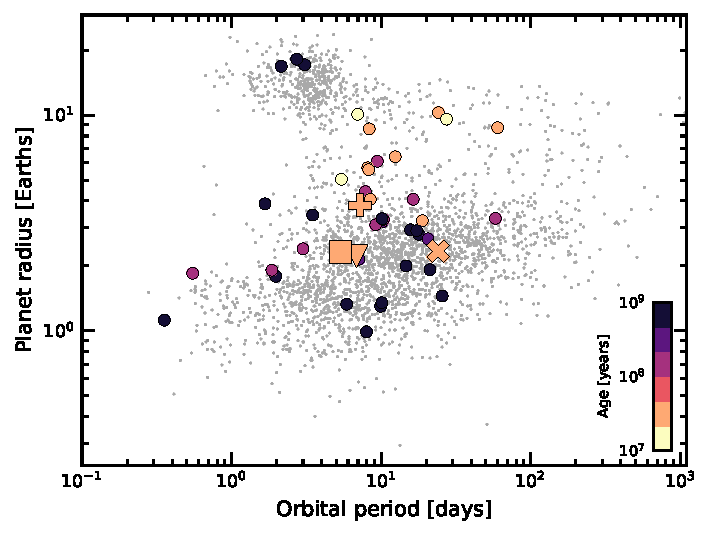
\includegraphics[width=0.9\textwidth]{f4.pdf}
	\end{center}
	\vspace{-0.7cm}
	\caption{
		%    namelist = ['Kepler-1627 A', 'KOI-7368', 'KOI-7913 A', 'KOI-7913 B', 'Kepler-1643']
		%    markers = ['P', 'v', 'X', 'X', 's']
		{\bf Radii, orbital periods, and ages of transiting exoplanets}.
    Planets younger than a gigayear with ${\rm \tau}/\sigma_{\tau} >
    3$ are emphasized, where $\tau$ is the age and $\sigma_{\tau}$ is
    its uncertainty. Kepler-1627 (+), KOI-7368 (down-triangle),
    KOI-7913 (X), Kepler-1643 (diamond).  The large sizes of the
    youngest transiting planets could be tied to a selection effect.
    Kepler-1643, KOI-7368, and KOI-7913 have normal mini-Neptune sizes
    of 2 to 3\,$R_\oplus$, which is a novelty given their ages.
    Parameters are from the NASA Exoplanet Archive (2022 Apr 5).
		\label{fig:rp_period_age}
	}
\end{figure*}


\subsection{Is CH-2 really a star cluster?}

RSG-5, and Kepler-1643's membership inside it, clearly meet the
typical expectations of a star claimed to be in an open cluster.
RSG-5 shows an obvious overdensity relative to the local field
population ({\it e.g.}, Figure~\ref{fig:XYZvtang}), and our membership
selection easily produces a clean pre-main-sequence locus in 
color-absolute magnitude space (Figure~\ref{fig:age}).
CH-2, and KOI-7913 and KOI-7368's membership inside it, do not meet
those expectations in as obvious a manner.  This is because this
association of stars is diffuse.

%really 80:9
To quantify the density discrepancy, we can compare the spatial and
velocity volumes searched to select candidate members of each cluster.
For RSG-5, we drew 141 candidate members from a $30\,{\rm
pc}\times30\,{\rm pc}\times30\,{\rm pc}$ spatial cube, given a $1 {\rm \mkms} \times 2 {\rm \mkms }$ rectangle in apparent galactic velocity.
For CH-2, our 37 candidate members came from a spatial cube of
dimension $50\,{\rm pc}\times40\,{\rm pc}\times30\,{\rm pc}$, and the
velocity rectangle of $2 {\rm \mkms} \times 4 {\rm \mkms}$.  If we
define the ``searched volume'' in units of ${\rm pc}^3 {\rm
(\mkms)}^2$, then the volume ratio of CH-2:RSG-5 is $\approx$9:1.  The
density (number of stars per unit searched volume) within RSG-5 relative to
CH-2 similarly comes out to 34 to 1.

So what makes a star cluster?  Historic answers to this question have
recently by reviewed by \citet{krumholz_star_2019}: some definitions
that have been offered include criteria such as being gravitationally
bound, and having a mass density that significantly exceeds the mean
in a cluster's galactic neighborhood.  We prefer a modified version of
the definition adopted by \citet{krumholz_star_2019}: for our purposes
a star cluster is a group of at least 12 stars that was physically
associated at its time of formation.  The somewhat arbitrary ``12'' is
set to distinguish clusters from high-order multiple star systems.  We
therefore explicitly include dissolved clusters and their tidal tails
in our concept of clusters.  We also explicitly exclude the idea that
a particular number of stars per unit spatial volume is required to
define a cluster.  The latter point acknowledges the fact that an
important factor in cluster identification is now also the number per
unit velocity volume, whether in 2-dimensional tangential velocity, or
when including the third radial component.  Perhaps
once stellar rotation periods and chemical abundances reach the same
level of ubiquity as stellar proper motions, they might enable further
refinement of our ability in cluster discovery.

From a data-driven perspective, how do we demonstrate that a star is
in a cluster, {\it i.e.}, that it is part of a group of stars that was
physically associated at its time of formation?
Back-integrating the orbits is one convincing approach, but it does
not always work {\bf (CITE)}.
The relatively minimal approach suggested by \citet{tofflemire_2021}
is intriguing: search for coeval, phase-space neighbors, measure their
ages, and determine if they share a common age.
This approach is more accurately be described as a method for
determining whether a star is currently associated with a set of coeval
stars, which is much easier to determine than what the association
looked like in the past.
From this standard, our analysis thus far of CH-2 has already
demonstrated the existence of such an assocation.

A crucial logical step in this method however is to ensure that the
(automated) search process for coeval phase-space neighbors in fact
produces neighbors at a rate different from what it would for field
stars.

% TODO
And so we ask: what is the density of field stars in the CH-2 region?
If we had applied Ronan's pre-main-sequence selection, + HDBScan, +
local neighbors... what would we have gotten?
Similarly... if you just applied Adam Kraus' Comove 
What is the likelihood we are fooling ourselves?


\subsection{Normal-Sized Mini-Neptunes Exist at 40$\,$Myr}

In the context of the existing exoplanet population, the most significant
novelty about Kepler-1643~b, KOI-7368.01, and KOI-7913 is that they have normal
mini-Neptune sizes.
More specifically, the intrinsic distribution of planet sizes measured
by Kepler peaks at $\approx 2.4\,R_\oplus$, with a valley at
1.8\,$R_\oplus$, and falling off past $\approx$3.5\,$R_\oplus$
\citep[][Figure~7]{Fulton_et_al_2017}.

Figure~\ref{fig:rp_period_age} shows the sizes, orbital periods, and ages of
known transiting planets, emphasizing those with precise ages.
Considering planets younger than $10^8$ years, the smallest previously
known were AU~Mic~c ($\approx3.0\pm0.2\,R_\oplus$, averaging the
results of \citealt{martioli_aumicbc_2021} and
\citealt{gilbert_flares_2022}), Kepler-1627~Ab ($3.8\pm0.2\,R_\oplus$;
\citealt{bouma_kep1627_2022}), and AU~Mic~d ($4.2\pm0.2\,R_\oplus$;
\citealt{plavchan_planet_2020}).
The other transiting planets younger than $10^8$ years are much
larger, with sizes between 4 and 10$\,R_\oplus$
\citep{Mann_K2_33b_2016,David_et_al_2017,benatti_possibly_2019,david_four_2019,newton_tess_2019,rizzuto_tess_2020,bouma_cluster_2020}.







\subsection{Summary}

We have argued that Kepler-1643~b, KOI-7368.01, and KOI-7913 {\it i)}
are 40 to 50 million years old, and {\it ii)} that each signal
is most likely planetary.  The evidence for the planetary
interpretation comes from an application of \texttt{VESPA} to the
Kepler data, alongside new adaptive optics imaging from NIRC2.  The
validity of the \texttt{VESPA} framework rests on the premise that
non-astrophysical false positives, including false alarms and known
neighboring eclipsing binaries, can be rejected.  Kepler-1643 and
KOI-7368 both pass all but one of the canonical vetting checks: the
check for centroid offsets between the in and out-of-transit phases.
For both cases, we have argued the weak observed shifts are most
likely caused by starspot-induced variability in specific quarters
shifting the stellar center-of-light.

Each system has multiple indicators of youth that support the
reported ages.  For Kepler-1643, perhaps the strongest youth indicator
is its physical and kinematic association with RSG-5.  Based on the
color-absolute magnitude diagram, we are able to select members
of this cluster with a false positive rate of $\ll 5\%$
(Figure~\ref{fig:age}); Kepler-1643 is one such member.  The stellar
rotation period period agrees with this assessment, and {\bf its
lithium is a little low}.

The spatio-kinematic argument for the youth of KOI-7368 and
KOI-7913 are weaker because they are in an association of stars, CH-2,
that is more diffuse.  For KOI-7913, stronger indicators of its age
perhaps come from its binary.  Both stellar components in KOI-7913
have isochronal ages consistent with $40$\,Myr, but the isochronal
measurement for the secondary is more constraining since it is less
massive.  Both components also show H$\alpha$ in emission, which for
the $\approx$K6V primary is a good indicator that the star is
$\lesssim$100$\,$Myr old.  For KOI-7368, which is slightly more
massive, the Li 6708\AA\ EW measurement and stellar rotation period
are more constraining, and provide independent verification of the
star's youth.





%%%%%%%%%%%%%%%%%%%%%%%%%%%%%%%%%%%%%%%%%%%%%%%%%%%%%%%%%%%%%%%%%%%%%%%%%%%%%%%


%\clearpage
\acknowledgements
\raggedbottom
%
L.G.B{.} acknowledges support from the TESS GI Program (NASA grants
80NSSC19K0386 and 80NSSC19K1728) and the Heising-Simons Foundation (51 Pegasi~b
Fellowship).
% programs G011103 and G022117, through 
%
%
%FIXME
Keck/NIRC2 imaging was acquired by program 2015A/N301N2L
(PI: A.~Kraus). % and 2019A/N069 (PI: E.~Petigura).
%
% ACKNOWLEDGE PFS / CAMPANAS.
%
This paper also includes data collected by the TESS mission, which are
publicly available from the Mikulski Archive for Space Telescopes
(MAST).
%
Funding for the TESS mission is provided by NASA's Science Mission
directorate.
%
We thank the TESS Architects (G.~Ricker, R.~Vanderspek, D.~Latham,
S.~Seager, J.~Jenkins) and the many TESS team members for their
efforts to make the mission a continued success.
%
%
%This study was based in part on observations at Cerro Tololo
%Inter-American Observatory at NSF's NOIRLab (NOIRLab Prop{.} ID
%2020A-0146; 2020B-0029 PI: Bouma), which is managed by the
%Association of Universities for Research in Astronomy (AURA) under a
%cooperative agreement with the National Science Foundation.
%
%
%Finally, this research has made use of the Keck Observatory Archive (KOA),
%which is operated by the W. M. Keck Observatory and the NASA Exoplanet
%Science Institute (NExScI), under contract with the National
%Aeronautics and Space Administration.
Finally, we also thank the Keck Observatory staff for their support of
HIRES and remote observing.  We recognize the importance that the
summit of Maunakea has within the indigenous Hawaiian community, and
are deeply grateful to have the opportunity to conduct observations
from this mountain.
%
% The Digitized Sky Survey was produced at the Space Telescope Science
% Institute under U.S. Government grant NAG W-2166.
% Figure~\ref{fig:scene} is based on photographic data obtained using
% the Oschin Schmidt Telescope on Palomar Mountain.
%

% %
% This research made use of the NASA Exoplanet Archive, which is
% operated by the California Institute of Technology, under contract
% with the National Aeronautics and Space Administration under the
% Exoplanet Exploration Program.
% %

% Resources supporting this work were provided by the NASA High-End
% Computing (HEC) Program through the NASA Advanced Supercomputing (NAS)
% Division at Ames Research Center for the production of the SPOC data
% products.
%

% A.J.\ and R.B.\ acknowledge support from project IC120009 ``Millennium
% Institute of Astrophysics (MAS)'' of the Millenium Science Initiative,
% Chilean Ministry of Economy. A.J.\ acknowledges additional support
% from FONDECYT project 1171208.  J.I.V\ acknowledges support from
% CONICYT-PFCHA/Doctorado Nacional-21191829.  R.B.\ acknowledges support
% from FONDECYT Post-doctoral Fellowship Project 3180246.
% %
% C.T.\ and C.B\ acknowledge support from Australian Research Council
% grants LE150100087, LE160100014, LE180100165, DP170103491 and
% DP190103688.
% %
% C.Z.\ is supported by a Dunlap Fellowship at the Dunlap Institute for
% Astronomy \& Astrophysics, funded through an endowment established by
% the Dunlap family and the University of Toronto.
% %
% D.D.\ acknowledges support through the TESS Guest Investigator Program
% Grant 80NSSC19K1727.
%
%
%
% %
% Based on observations obtained at the Gemini Observatory, which is
% operated by the Association of Universities for Research in Astronomy,
% Inc., under a cooperative agreement with the NSF on behalf of the
% Gemini partnership: the National Science Foundation (United States),
% National Research Council (Canada), CONICYT (Chile), Ministerio de
% Ciencia, Tecnolog\'{i}a e Innovaci\'{o}n Productiva (Argentina),
% Minist\'{e}rio da Ci\^{e}ncia, Tecnologia e Inova\c{c}\~{a}o (Brazil),
% and Korea Astronomy and Space Science Institute (Republic of Korea).
% %
% Observations in the paper made use of the High-Resolution Imaging
% instrument Zorro at Gemini-South. Zorro was funded by the NASA
% Exoplanet Exploration Program and built at the NASA Ames Research
% Center by Steve B. Howell, Nic Scott, Elliott P. Horch, and Emmett
% Quigley.
% %
% This research has made use of the VizieR catalogue access tool, CDS,
% Strasbourg, France. The original description of the VizieR service was
% published in A\&AS 143, 23.
% %
% This work has made use of data from the European Space Agency (ESA)
% mission {\it Gaia} (\url{https://www.cosmos.esa.int/gaia}), processed
% by the {\it Gaia} Data Processing and Analysis Consortium (DPAC,
% \url{https://www.cosmos.esa.int/web/gaia/dpac/consortium}). Funding
% for the DPAC has been provided by national institutions, in particular
% the institutions participating in the {\it Gaia} Multilateral
% Agreement.
%
% (Some of) The data presented herein were obtained at the W. M. Keck
% Observatory, which is operated as a scientific partnership among the
% California Institute of Technology, the University of California and
% the National Aeronautics and Space Administration. The Observatory was
% made possible by the generous financial support of the W. M. Keck
% Foundation.
% The authors wish to recognize and acknowledge the very significant
% cultural role and reverence that the summit of Maunakea has always had
% within the indigenous Hawaiian community.  We are most fortunate to
% have the opportunity to conduct observations from this mountain.
%
% \newline
%

\software{
  %\texttt{arviz} \citep{arviz_2019},
  %\texttt{altaipony} \citep{ilin_flares_2021},
  \texttt{astrobase} \citep{bhatti_astrobase_2018},
  %\texttt{astroplan} \citep{astroplan2018},
	%\texttt{AstroImageJ} \citep{collins_astroimagej_2017},
  \texttt{astropy} \citep{astropy_2018},
  \texttt{astroquery} \citep{astroquery_2018},
  %\texttt{BATMAN} \citep{kreidberg_batman_2015},
  %\texttt{ceres} \citep{brahm_2017_ceres},
  %\texttt{cdips-pipeline} \citep{bhatti_cdips-pipeline_2019},
  %\texttt{corner} \citep{corner_2016},
  %\texttt{emcee} \citep{foreman-mackey_emcee_2013},
  \texttt{exoplanet} \citep{exoplanet:exoplanet}, and its
  dependencies \citep{exoplanet:agol20, exoplanet:kipping13, exoplanet:luger18,
   	exoplanet:theano},
	%\texttt{gala} \citep{gala,PriceWhelan_2017_gala_zenodo},
	%\texttt{IDL Astronomy User's Library} \citep{landsman_1995},
  %\texttt{IPython} \citep{perez_2007},
	%\texttt{isochrones} \citep{morton_2015_isochrones},
	%\texttt{lightkurve} \citep{lightkurve_2018},
  %\texttt{matplotlib} \citep{hunter_matplotlib_2007}, 
  %\texttt{MESA} \citep{paxton_modules_2011,paxton_modules_2013,paxton_modules_2015}
  %\texttt{numpy} \citep{walt_numpy_2011}, 
  %\texttt{pandas} \citep{mckinney-proc-scipy-2010},
  %\texttt{pyGAM} \citep{serven_pygam_2018_1476122},
  \texttt{PyMC3} \citep{salvatier_2016_PyMC3},
  %\texttt{radvel} \citep{fulton_radvel_2018},
  %\texttt{scikit-learn} \citep{scikit-learn},
  \texttt{scipy} \citep{jones_scipy_2001},
  %\texttt{TESS-point}  \citep{burke_2020},
  %\texttt{tesscut} \citep{brasseur_astrocut_2019},
	\texttt{VESPA} \citep{morton_efficient_2012,vespa_2015},
  %\texttt{webplotdigitzer} \citep{rohatgi_2019},
  %\texttt{wotan} \citep{hippke_wotan_2019}.
}
\ 

\facilities{
 	{\it Astrometry}:
 	Gaia \citep{gaia_collaboration_gaia_2018,gaia_collaboration_2021_edr3}.
 	{\it Imaging}:
    Second Generation Digitized Sky Survey. %,
    %SOAR~(HRCam; \citealt{tokovinin_ten_2018}).
 	Keck:II~(NIRC2; \url{www2.keck.hawaii.edu/inst/nirc2}).
 	%Gemini:South~(Zorro; \citealt{scott_nessi_2018}.
 	%Gemini:North~(`Alopeke; \citealt{scott_nessi_2018,scott_twin_2021}.
 	{\it Spectroscopy}:
	%CTIO1.5$\,$m~(CHIRON; \citealt{tokovinin_chironfiber_2013}),
  %PFS ({\bf CITE}),
	Tillinghast:1.5m~(TRES; \citealt{furesz_tres_2008}).
  %MPG2.2$\,$m~(FEROS; \citealt{kaufer_commissioning_1999}),
	%AAT~(Veloce; \citealt{gilbert_veloce_2018}).
	%AAT~(HERMES; \citealt{lewis_2002_hermers_2df,sheinis_2015_hermes}),
 	Keck:I~(HIRES; \citealt{vogt_hires_1994}).
 	%VLT:Kueyen~(FLAMES; \citealt{pasquini_2002}).
% 	Euler1.2m~(CORALIE),
% 	ESO:3.6m~(HARPS; \citealt{mayor_setting_2003}).
 	{\it Photometry}:
%	  ASTEP:0.40$\,$m (ASTEP400),
% 	CTIO:1.0m (Y4KCam),
% 	Danish 1.54m Telescope,
%	  El Sauce:0.356$\,$m,
% 	Elizabeth 1.0m at SAAO,
% 	Euler1.2m (EulerCam),
	  Kepler \citep{borucki_kepler_2010},
% 	Magellan:Baade (MagIC),
% 	Max Planck:2.2m	(GROND; \citealt{greiner_grond7-channel_2008})
%   MuSCAT3 \citep{Narita_2020},
% 	NTT,
% 	SOAR (SOI),
 	  TESS \citep{ricker_transiting_2015}.
% 	TRAPPIST \citep{jehin_trappist_2011},
% 	VLT:Antu (FORS2).
}

% \begin{table*}
\scriptsize
\setlength{\tabcolsep}{2pt}
\centering
\caption{Literature and Measured Properties for Kepler$\,$1627}
\label{tab:starparams}
%\tablenum{2}
\begin{tabular}{llcc}
  \hline
  \hline
Primary Star\dotfill & \\
\multicolumn{3}{c}{TIC 120105470} \\
\multicolumn{3}{c}{GAIADR2$^\dagger$ 2103737241426734336} \\
\hline
\hline
Parameter & Description & Value & Source\\
\hline 
$\alpha_{J2015.5}$\dotfill	&Right Ascension (hh:mm:ss)\dotfill & 18:56:13.6 & 1	\\
$\delta_{J2015.5}$\dotfill	&Declination (dd:mm:ss)\dotfill & +41:34:36.22 & 1	\\
%
V\dotfill			&Johnson V mag.\dotfill & 13.11 $\pm$ 0.08		& 2	\\
${\rm G}$\dotfill     & Gaia $G$ mag.\dotfill     & 13.02$\pm$0.02 & 1\\
$G_{\rm BP}$\dotfill     & Gaia $BP$ mag.\dotfill     & 13.43$\pm$0.02 & 1\\
$G_{\rm RP}$\dotfill     & Gaia $RP$ mag.\dotfill     & 12.44$\pm$0.02 & 1\\
${\rm T}$\dotfill     & TESS $T$ mag.\dotfill     & 12.53$\pm$0.02 & 2\\
J\dotfill			& 2MASS J mag.\dotfill & 11.69  $\pm$ 0.02	& 3	\\
H\dotfill			& 2MASS H mag.\dotfill & 11.30 $\pm$ 0.02	    &  3	\\
K$_{\rm S}$\dotfill			& 2MASS ${\rm K_S}$ mag.\dotfill & 11.19 $\pm$ 0.02 &  3	\\
%
$\pi$\dotfill & Gaia EDR3 parallax (mas) \dotfill & 3.009 $\pm$ 0.032 &  1 \\
$d$\dotfill & Distance (pc)\dotfill & $329.5 \pm 3.5$ & 1, 4 \\
$\mu_{\alpha}$\dotfill		& Gaia EDR3 proper motion\dotfill & 1.716 $\pm$ 0.034 & 1 \\
                    & \hspace{3pt} in RA (mas yr$^{-1}$)	&  \\
$\mu_{\delta}$\dotfill		& Gaia EDR3 proper motion\dotfill 	&  -1.315 $\pm$ 0.034 &  1 \\
                    & \hspace{3pt} in DEC (mas yr$^{-1}$) &  \\
RUWE\dotfill		& Gaia EDR3 renormalized\dotfill 	&  2.899 &  1 \\
                    & \hspace{3pt} unit weight error &  \\
RV\dotfill & Systemic radial \hspace{9pt}\dotfill  & $-16.7 \pm 1.0$ & 5 \\
                    & \hspace{3pt} velocity (\kms)  & \\
%
Spec. Type\dotfill & Spectral Type\dotfill & 	G8V & 5 \\
$v\sin{i_\star}$\dotfill &  Rotational velocity$^*$ (\kms) \hspace{9pt}\dotfill &  18.9 $\pm$ 1.0 & 5 \\
Li EW\dotfill & 6708\AA\ Equiv{.} Width (m\AA) \dotfill & $233^{+5}_{-7}$  & 5 \\
$T_{\rm eff}$\dotfill &  Effective Temperature (K) \hspace{9pt}\dotfill & 5505 $\pm$ 60 &  6  \\
$\log{g_{\star}}$\dotfill &  Surface Gravity (cgs)\hspace{9pt}\dotfill &  4.53 $\pm$ 0.05  &  6 \\
$R_\star$\dotfill & Stellar radius ($R_\odot$)\dotfill & 0.881$\pm$0.018 & 6 \\
$M_\star$\dotfill & Stellar mass ($R_\odot$)\dotfill & 0.953$\pm$0.019 & 6 \\
$A_{\rm V}$\dotfill & Interstellar reddening (mag)\dotfill & 0.2 $\pm$ 0.1 & 6 \\
${\rm [Fe/H]}$\dotfill &   Metallicity\dotfill & 0.1 $\pm$ 0.1 & 6 \\
%
$P_{\rm rot}$\dotfill & Rotation period (d)\dotfill & $2.642\pm 0.042$  & 7 \\
Age & Adopted stellar age (Myr)\dotfill & $38^{+6}_{-5}$  &  8 \\
%
\hline 
%
$\Delta m_{832}$ & Mag difference (`Alopeke 832\,nm)\dotfill & $3.14 \pm 0.04$ & 9 \\
$\theta_{\rm B}$ & Position angle (deg)\dotfill & $91.9 \pm 0.7$ & 9 \\
$\rho_{\rm B}$ & Apparent separation of \dotfill & $0.164 \pm 0.010$ &  9 \\
                    & \hspace{3pt} primary and secondary (as) &  \\
$\rho_{\rm B}$ & Apparent separation of \dotfill & $53 \pm 4$ &  1,4,9 \\
                    & \hspace{3pt} primary and secondary (AU) &  \\
$\Delta m_{K'}$ & Mag difference (NIRC2 $K'$)\dotfill & $2.37 \pm 0.02$ & 10 \\
$\theta_{\rm B}$ & Position angle (deg)\dotfill & $95.9 \pm 0.5$ & 10 \\
$\rho_{\rm B}$ & Apparent separation of \dotfill & $0.1739 \pm 0.0017$ &  10 \\
                    & \hspace{3pt} primary and secondary (as) &  \\
%
\hline
\end{tabular}
\begin{flushleft}
 \footnotesize{ \textsc{NOTE}---
 $^\dagger$ The GAIADR2 and GAIAEDR3 identifiers for Kepler 1627A are identical.  The secondary
 is not resolved in the Gaia point source catalog.
 $^*$ Given only $v\sin i$ and $2\piR_\star/P_{\rm rot}$, $\cos i=0.11^{+0.11}_{-0.08}$.
Provenances are:
$^1$\citet{gaia_collaboration_2021_edr3},
$^2$\citet{stassun_TIC8_2019},
$^3$\citet{skrutskie_tmass_2006},
$^4$\citet{Lindegren_2021_offset},
$^5$HIRES spectra and \citet{yee_SM_2017},
$^6$Cluster isochrone (MIST adopted; PARSEC compared for quoted
  uncertainty),
$^7$Kepler light curve,
$^8$Pre-main-sequence CAMD interpolation (Section~\ref{sec:camd}),
$^9$`Alopeke imaging 2021 June 24 \citep{scott_twin_2021},
$^{10}$NIRC2 imaging 2015 July 22.
}
\end{flushleft}
\vspace{-0.5cm}
\end{table*}

% % Table of best fit parameters
%\startlongtable
\begin{deluxetable*}{lllrrrrrrr}
%
  \tablecaption{ Priors and posteriors for the transit and stellar
  variability model fitted to the long-cadence Kepler 1627b
  photometric timeseries.}
\label{tab:posterior}
%
\tabletypesize{\scriptsize}
%\tabletypesize{\small}
%
%\tablenum{2}
%
\tablehead{
  \colhead{Param.} & 
  \colhead{Unit} &
  \colhead{Prior} & 
  \colhead{Median} & 
  \colhead{Mean} & 
  \colhead{Std{.} Dev.} &
  \colhead{3\%} &
  \colhead{97\%} &
  \colhead{ESS} &
  \colhead{$\hat{R}-1$}
}

%/Users/luke/Dropbox/proj/rudolf/results/run_RotStochGPtransit/Kepler_1627_RotStochGPtransit_posteriortable.tex
\startdata
{\it Sampled} & & & & & & & & & \\
\hline
$P$ & d & $\mathcal{N}(7.20281; 0.01000)$ & 7.2028035 & 7.2028033 & 0.0000073 & 7.2027893 & 7.2028171 & 1910.5903732 & 0.0035905 \\
$t_0^{(1)}$ & d & $\mathcal{N}(120.79053; 0.02000)$ & 120.790504 & 120.790505 & 0.0009438 & 120.7886867 & 120.7922431 & 1564.1105056 & 0.0003213 \\
$\log R_{\rm p}/R_\star$ & -- & $\mathcal{U}(-4.605; 0.000)$ & -3.33523 & -3.33569 & 0.06618 & -3.45772 & -3.21617 & 1173.56574 & 0.00310 \\
$b$ & -- & $\mathcal{U}(0; 1+R_{\mathrm{p}}/R_\star)$ & 0.3971 & 0.3886 & 0.2070 & 0.0204 & 0.7289 & 378.9528 & 0.0177 \\
$u_1$ & -- & \citet{exoplanet:kipping13} & 0.28 & 0.30 & 0.179 & 0.002 & 0.603 & 1161.95 & 0.005 \\
$u_2$ & -- & \citet{exoplanet:kipping13} & 0.425 & 0.381 & 0.314 & -0.197 & 0.912 & 900.884 & 0.002 \\
$R_\star$ & $R_\odot$ & $\mathcal{T}(0.910; 0.052)$ & 0.911 & 0.910 & 0.051 & 0.814 & 1.004 & 2265.830 & -0.001 \\
$\log g$ & cgs & $\mathcal{N}(4.600; 0.100)$ & 4.604 & 4.601 & 0.094 & 4.417 & 4.769 & 923.943 & 0. \\
$\langle f \rangle$ & -- & $\mathcal{N}(0.500; 0.100)$ & 0.4999 & 0.4999 & 0.0003 & 0.4993 & 0.5005 & 2964.6676 & 0.0013 \\
$e^{(2)}$ & -- & \citet{vaneylen19} & 0.127 & 0.168 & 0.147 & 0. & 0.446 & 518.492 & 0.004 \\
$\omega$ & rad & $\mathcal{U}(0.000; 6.283)$ & -0.235 & -0.170 & 1.867 & -2.879 & 3.132 & 1212.260 & 0.006 \\
$\log \sigma_f$ & -- & $\mathcal{N}(\log\langle \sigma_f \rangle; 2.000)$ & -8.016 & -8.016 & 0.008 & -8.031 & -8.001 & 2224.427 & -0. \\
$\rho$ & d & $\mathcal{U}(1.000; 10.000)$ & 2.953 & 2.955 & 0.096 & 2.777 & 3.131 & 1936.492 & 0. \\
$\sigma$ & d$^{-1}$ & $\mathrm{InvGamma}(1.000; 5.000)$ & 0.013 & 0.013 & 0.001 & 0.012 & 0.014 & 2155.687 & -0. \\
$\sigma_{\mathrm{rot}}$ & d$^{-1}$ & $\mathrm{InvGamma}(1.000; 5.000)$ & 0.897 & 0.933 & 0.222 & 0.552 & 1.316 & 2147.324 & 0.003 \\
$\log P_{\mathrm{rot}}$ & $\log (\mathrm{d})$ & $\mathcal{N}(0.958; 0.020)$ & 0.964 & 0.964 & 0.001 & 0.963 & 0.966 & 2486.029 & 0. \\
$\log Q_0$ & -- & $\mathcal{N}(0.000; 2.000)$ & 12.935 & 12.960 & 0.454 & 12.157 & 13.857 & 2126.581 & 0.004 \\
$\log \mathrm{d}Q$ & -- & $\mathcal{N}(0.000; 2.000)$ & 0.029 & 0.021 & 2.032 & -3.785 & 3.780 & 1755.941 & 0. \\
$f$ & -- & $\mathcal{U}(0.100; 1.000)$ & 0.111 & 0.113 & 0.010 & 0.1 & 0.130 & 1253.358 & -0.0 \\
\hline
{\it Derived} & & & & & & & & & \\
\hline
$R_{\rm p}/R_\star$ & -- & -- & 0.036 & 0.036 & 0.002 & 0.031 & 0.040 & 1173.566 & 0.003 \\
$\rho_\star$ & g$\ $cm$^{-3}$ & -- & 2.27 & 2.312 & 0.516 & 1.408 & 3.272 & 910.746 & 0.001 \\
$R_{\rm p}$ & $R_{\mathrm{Jup}}$ & -- & 0.316 & 0.317 & 0.037 & 0.251 & 0.386 & 1692.736 & 0.001 \\
$a/R_\star$ & -- & -- & 18.396 & 18.407 & 1.375 & 15.690 & 20.780 & 910.717 & 0.001 \\
$\cos i$ & -- & -- & 0.022 & 0.021 & 0.011 & 0.002 & 0.038 & 439.303 & 0.011 \\
$T_{14}$ & hr & -- & 2.822 & 2.823 & 0.057 & 2.710 & 2.917 & 1086.008 & 0.002 \\
$T_{13}$ & hr & -- & 2.578 & 2.566 & 0.083 & 2.430 & 2.714 & 590.630 & 0.011 \\
\enddata
%
\tablecomments{
  ESS refers to the number of effective samples.
  $\hat{R}$ is the Gelman-Rubin convergence diagnostic.
  Logarithms through this table are in base-$e$.
  $\mathcal{U}$ denotes a uniform distribution,
  $\mathcal{N}$ a normal distribution, and
  $\mathcal{T}$ a truncated normal bounded between zero and an upper limit much larger than the mean.
  (1) The ephemeris is in units of BJDTDB - 2454833.
  (2) The eccentricity vectors are sampled in the $(e\cos\omega,
  e\sin\omega)$ basis.
%
% (2) Uninformative quadratic limb-darkening prior from \citet{exoplanet:kipping13}, implemented by \citet{exoplanet:exoplanet}.
% The precision achieved in the ground-based data did not appear to
% necessitate using bandpass-dependent limb-darkening coefficients.
% For comparison, the \citet{claret_limb_2017} parameters for
% the appropriate $T_{\rm eff}$ and $\log g$ in TESS-band would have been 
% $(u_1, u_2) = (0.3249, 0.235)$.
%
% (2) Assuming an informative quadratic limb-darkening prior with
% values about those given for the appropriate $T_{\rm eff}$ and
% $\log g$ in TESS-band from \citet{claret_limb_2017}. The precision
% achieved in the ground-based data did not appear to necessitate using
% bandpass-dependent limb-darkening coefficients.
% (3) The second and third contact points do not exist for a grazing transit.
% {\it Notation}:
% $a_{ij;\mathrm{Instr}}$ denotes the $i^{\rm th}$ transit of a
% particular instrument, and the $j^{\rm th}$ polynomial detrending
% order.
}
\vspace{-0.3cm}
\end{deluxetable*}

% %% \begin{deluxetable}{} command tell LaTeX how many columns
%% there are and how to align them.
%\startlongtable
\begin{deluxetable*}{lll}
    
%% Keep a portrait orientation

%% Over-ride the default font size
%% Use Default (12pt)
\tabletypesize{\scriptsize}
%\tabletypesize{\small}

%% Use \tablewidth{?pt} to over-ride the default table width.
%% If you are unhappy with the default look at the end of the
%% *.log file to see what the default was set at before adjusting
%% this value.

%% This is the title of the table.
\tablecaption{Young, Age-dated, and Age-dateable Stars Within the
  Nearest Few Kiloparsecs ($\texttt{v0.5}$ of the CDIPS Target
  List).}
\label{tab:v05}

%% This command over-rides LaTeX's natural table count
%% and replaces it with this number.  LaTeX will increment 
%% all other tables after this table based on this number
%\tablenum{3}

%% The \tablehead gives provides the column headers.  It
%% is currently set up so that the column labels are on the
%% top line and the units surrounded by ()s are in the 
%% bottom line.  You may add more header information by writing
%% another line between these lines. For each column that requries
%% extra information be sure to include a \colhead{text} command
%% and remember to end any extra lines with \\ and include the 
%% correct number of &s.
\tablehead{
  \colhead{Parameter} &
  \colhead{Example Value} &
  \colhead{Description}
}

%% All data must appear between the \startdata and \enddata commands
%
% paste from
% /Users/luke/Dropbox/proj/rudolf/results/tables/v05_main_tableheader.tex
% via drivers/write_v05_main_tableheader.py
\startdata
         \texttt{source\_id} &                                         1709456705329541504 &                                             Gaia DR2 source identifier. \\
                 \texttt{ra} &                                                     247.826 &                                         Gaia DR2 right ascension [deg]. \\
                \texttt{dec} &                                                      79.789 &                                             Gaia DR2 declination [deg]. \\
           \texttt{parallax} &                                                      35.345 &                                                Gaia DR2 parallax [mas]. \\
    \texttt{parallax\_error} &                                                       0.028 &                                    Gaia DR2 parallax uncertainty [mas]. \\
               \texttt{pmra} &                                                      94.884 &     Gaia DR2 proper motion $\mu_\alpha \cos \delta$ [mas$\,$yr${^-1}$]. \\
              \texttt{pmdec} &                                                     -86.971 &                 Gaia DR2 proper motion $\mu_\delta$ [mas$\,$yr${^-1}$]. \\
 \texttt{phot\_g\_mean\_mag} &                                                        6.85 &                                                 Gaia DR2 $G$ magnitude. \\
\texttt{phot\_bp\_mean\_mag} &                                                       6.409 &                                     Gaia DR2 $G_\mathrm{BP}$ magnitude. \\
\texttt{phot\_rp\_mean\_mag} &                                                       7.189 &                                     Gaia DR2 $G_\mathrm{RP}$ magnitude. \\
            \texttt{cluster} &                 Uma,IR\_excess,NASAExoArchive\_ps\_20210506 &                                  Comma-separated cluster or group name. \\
                \texttt{age} &                                                nan,nan,9.48 & Comma-separated logarithm (base-10) of reported$^{\rm a}$ age in years. \\
          \texttt{mean\_age} &                                                        9.48 &                          Mean (ignoring NaNs) of $\texttt{age}$ column. \\
      \texttt{reference\_id} &      Ujjwal2020,CottenSong2016,NASAExoArchive\_ps\_20210506 &                          Comma-separted provenance of group membership. \\
 \texttt{reference\_bibcode} & 2020AJ....159..166U,2016ApJS..225...15C,2013PASP..125..989A &                  ADS bibcode corresponding to $\texttt{reference\_id}$. \\
\enddata

%% Include any \tablenotetext{key}{text}, \tablerefs{ref list},
%% or \tablecomments{text} between the \enddata and 
%% \end{deluxetable} commands

%% General table comment marker
\tablecomments{
Table~\ref{tab:v05} is
published in its entirety in a machine-readable format.   This table is a
concatenation of the studies listed in Table~\ref{tab:metadata}.
One entry is
shown for guidance regarding form and content. 
In this particular example, the star has a
cold Jupiter on a 16 year orbit, HD 150706b \citep{2012AA...545A..55B}.
An infrared excess has been reported \citep{CottenSong2016}, and the star was identified by \citet{Ujjwal2020} as a candidate UMa moving group
member ($\approx 400\,{\rm Myr}$; \citealt{mann_tess_2020}).
The star's RV activity and TESS rotation period corroborate its youth.
}
\vspace{-0.5cm}
\end{deluxetable*}

% %% \begin{deluxetable}{} command tell LaTeX how many columns
%% there are and how to align them.
%\startlongtable
\begin{deluxetable*}{lccc}
    
%% Keep a portrait orientation

%% Over-ride the default font size
%% Use Default (12pt)
\tabletypesize{\scriptsize}
%\tabletypesize{\small}
%\tabletypesize{\normal}

%% Use \tablewidth{?pt} to over-ride the default table width.
%% If you are unhappy with the default look at the end of the
%% *.log file to see what the default was set at before adjusting
%% this value.

%% This is the title of the table.
\tablecaption{Provenances of Young and Age-dateable Stars.}
\label{tab:metadata}

%% This command over-rides LaTeX's natural table count
%% and replaces it with this number.  LaTeX will increment 
%% all other tables after this table based on this number
%\tablenum{3}

%% The \tablehead gives provides the column headers.  It
%% is currently set up so that the column labels are on the
%% top line and the units surrounded by ()s are in the 
%% bottom line.  You may add more header information by writing
%% another line between these lines. For each column that requries
%% extra information be sure to include a \colhead{text} command
%% and remember to end any extra lines with \\ and include the 
%% correct number of &s.
\tablehead{
  \colhead{Reference} &
  \colhead{$N_{\rm Gaia}$} &
  \colhead{$N_{\rm Age}$} &
  \colhead{$N_{G_{\rm RP}<16}$}
}

%% All data must appear between the \startdata and \enddata commands
%
% paste from
% /Users/luke/Dropbox/proj/rudolf/results/tables/metadata_table_data.tex
% via drivers/write_metadata_table.py
\startdata
                           \citet{Kounkel2020}  &             987376 &            987376 &                775363 \\
                     \citet{CantatGaudin2020a}  &             433669 &            412671 &                269566 \\
                     \citet{CantatGaudin2018a}  &             399654 &            381837 &                246067 \\
                      \citet{KounkelCovey2019}  &             288370 &            288370 &                229506 \\
                     \citet{CantatGaudin2020b}  &             233369 &            227370 &                183974 \\
                           \citet{Zari2018} UMS &              86102 &                 0 &                 86102 \\
                  \citet{SIMBAD} $\texttt{Y*?}$ &              61432 &                 0 &                 45076 \\
                           \citet{Zari2018} PMS &              43719 &                 0 &                 38435 \\
\citet{GaiaCollaboration2018} $d>250\,{\rm pc}$ &              35506 &             31182 &                 18830 \\
                      \citet{CastroGinard2020}  &              33635 &             24834 &                 31662 \\
                              \citet{Kerr2021}  &              30518 &             25324 &                 27307 \\
                  \citet{SIMBAD} $\texttt{Y*O}$ &              28406 &                 0 &                 16205 \\
                        \citet{VillaVelez2018}  &              14459 &             14459 &                 13866 \\
                     \citet{CantatGaudin2019a}  &              11843 &             11843 &                  9246 \\
                        \citet{Damiani2019} PMS &              10839 &             10839 &                  9901 \\
                                \citet{Oh2017}  &              10379 &                 0 &                 10370 \\
                          \citet{Meingast2021}  &               7925 &              7925 &                  5878 \\
                 \citet{SIMBAD} $\texttt{pMS*}$ &               5901 &                 0 &                  3006 \\
\citet{GaiaCollaboration2018} $d<250\,{\rm pc}$ &               5378 &               817 &                  3968 \\
                           \citet{Kounkel2018}  &               5207 &              3740 &                  5207 \\
                        \citet{Ratzenbock2020}  &               4269 &              4269 &                  2662 \\
                  \citet{SIMBAD} $\texttt{TT*}$ &               4022 &                 0 &                  3344 \\
                        \citet{Damiani2019} UMS &               3598 &              3598 &                  3598 \\
                           \citet{Rizzuto2017}  &               3294 &              3294 &                  2757 \\
            \citet{NASAExoArchive_ps_20210506}  &               3107 &               868 &                  3098 \\
                              \citet{Tian2020}  &               1989 &              1989 &                  1394 \\
                           \citet{Goldman2018}  &               1844 &              1844 &                  1783 \\
                        \citet{CottenSong2016}  &               1695 &                 0 &                  1693 \\
                            \citet{Gagne2018a}  &               1429 &                 0 &                  1389 \\
             \citet{RoserSchilbach2020} Psc-Eri &               1387 &              1387 &                  1107 \\
            \citet{RoserSchilbach2020} Pleiades &               1245 &              1245 &                  1019 \\
                  \citet{SIMBAD} $\texttt{TT?}$ &               1198 &                 0 &                   853 \\
                            \citet{Gagne2018c}  &                914 &                 0 &                   913 \\
                          \citet{Pavlidou2021}  &                913 &               913 &                   504 \\
                            \citet{Gagne2018b}  &                692 &                 0 &                   692 \\
                            \citet{Ujjwal2020}  &                563 &                 0 &                   563 \\
                             \citet{Gagne2020}  &                566 &               566 &                   351 \\
                      \citet{EsplinLuhman2019}  &                377 &               443 &                   296 \\
                     \citet{Roccatagliata2020}  &                283 &               283 &                   232 \\
                          \citet{Meingast2019}  &                238 &               238 &                   238 \\
                 \citet{Furnkranz2019} Coma-Ber &                214 &               214 &                   213 \\
           \citet{Furnkranz2019} Neighbor Group &                177 &               177 &                   167 \\
                             \citet{Kraus2014}  &                145 &               145 &                   145 \\
\enddata

%% Include any \tablenotetext{key}{text}, \tablerefs{ref list},
%% or \tablecomments{text} between the \enddata and 
%% \end{deluxetable} commands

%% General table comment marker
\tablecomments{
Table~\ref{tab:metadata} describes the provenances for the young and
age-dateable stars in Table~\ref{tab:v06}.  $N_{\rm Gaia}$: number of
Gaia stars we parsed from the literature source.  $N_{\rm Age}$:
number of stars in the literature source with ages reported.
$N_{G_{\rm RP}<16}$: number of Gaia stars we parsed from the
literature source with either $G_{\rm RP}<16$, or a parallax S/N
exceeding 5 and a distance closer than 100\,pc.  The latter criterion
included a few hundred white dwarfs that would have otherwise been
neglected.  Some studies are listed multiple times if they contain
multiple tables.  \citet{SIMBAD} refers to the \texttt{SIMBAD}
database.
}
\vspace{-0.5cm}
\end{deluxetable*}


\clearpage
\bibliographystyle{yahapj}                            
\bibliography{bibliography} 

\appendix
\section{Table of Candidate RSG-5 and CH-2 Members}
\label{app:members}

Gaia source lists and abbreviated info.  Include rotation periods.

\section{Table of Transit Fit Parameters}
\label{app:transit}

Tables~\ref{tab:kepler1643}, \ref{tab:koi7368}, \ref{tab:koi7913} give
the full set of fitted and derived parameters from the model described in
Section~\ref{sec:fitting}.
Priors and convergence statistics are also listed.

\begin{deluxetable*}{lllrrrrrrr}
	%
	\tablecaption{ Priors and posteriors for Kepler-1643 transit model with local
  polynomials removed.}
	\label{tab:kepler1643}
	%
	\tabletypesize{\scriptsize}
	%\tabletypesize{\small}
	%
	%\tablenum{2}
	%
	\tablehead{
		\colhead{Param.} & 
		\colhead{Unit} &
		\colhead{Prior} & 
		\colhead{Median} & 
		\colhead{Mean} & 
		\colhead{Std{.} Dev.} &
		\colhead{3\% HDI} &
		\colhead{97\% HDI} &
		\colhead{ESS} &
		\colhead{$\hat{R}-1$}
	}
  %
	\startdata
$P$ & d & $\mathcal{N}(5.34264; 0.01000)$ & 5.3426257 & 5.3426258 & 0.0000101 & 5.3426071 & 5.3426454 & 7884 & 1.1e-03 \\
$t_0^{(1)}$ & d & $\mathcal{N}(134.38100; 0.02000)$ & 134.3820412 & 134.3820408 & 0.0011172 & 134.3798834 & 134.3840798 & 7390 & 3.7e-04 \\
$\log R_{\rm p}/R_\star$ & -- & $\mathcal{U}(-6.215; 0.000)$ & -3.68806 & -3.68934 & 0.02072 & -3.72788 & -3.65275 & 4449 & -7.8e-05 \\
$b$ & -- & $\mathcal{U}(0; 1+R_{\mathrm{p}}/R_\star)$ & 0.5825 & 0.5781 & 0.0514 & 0.4848 & 0.6734 & 4705 & 1.9e-04 \\
$u_1$ & -- & Kipping 2013 & 0.257 & 0.294 & 0.214 & 0.000 & 0.678 & 5324 & 7.9e-04 \\
$u_2$ & -- & Kipping 2013 & 0.324 & 0.314 & 0.324 & -0.257 & 0.880 & 4908 & 8.4e-04 \\
$R_\star$ & $R_\odot$ & $\mathcal{N}(0.855; 0.044)$ & 0.851 & 0.851 & 0.045 & 0.766 & 0.933 & 7473 & 7.2e-04 \\
$\log g$ & cgs & $\mathcal{N}(4.502; 0.035)$ & 4.507 & 4.507 & 0.035 & 4.442 & 4.576 & 6530 & -1.4e-04 \\
$\log \sigma_f$ & -- & $\mathcal{N}(\log\langle \sigma_f \rangle; 2.000)$ & -8.520 & -8.520 & 0.019 & -8.556 & -8.486 & 7966 & 2.1e-04 \\
$\langle f \rangle$ & -- & $\mathcal{N}(1.000; 0.100)$ & 1.0000 & 1.0000 & 0.0000 & 1.0000 & 1.0000 & 7488 & 3.2e-04 \\
$R_{\rm p}/R_\star$ & -- & -- & 0.025 & 0.025 & 0.001 & 0.024 & 0.026 & 4449 & -7.8e-05 \\
$\rho_\star$ & g$\ $cm$^{-3}$ & -- & 1.943 & 1.953 & 0.191 & 1.603 & 2.313 & 6081 & 9.4e-05 \\
$R_{\rm p}$ & $R_{\mathrm{Jup}}$ & -- & 0.207 & 0.207 & 0.012 & 0.184 & 0.231 & 6326 & 2.5e-04 \\
$R_{\rm p}$ & $R_{\mathrm{Earth}}$ & -- & 2.32 & 2.32 & 0.135 & 2.062 & 2.589 & 6326 & 2.5e-04 \\
$a/R_\star$ & -- & -- & 14.312 & 14.322 & 0.465 & 13.487 & 15.228 & 6081 & 8.2e-05 \\
$\cos i$ & -- & -- & 0.041 & 0.040 & 0.005 & 0.032 & 0.049 & 4929 & 2.4e-04 \\
$T_{14}$ & hr & -- & 2.408 & 2.409 & 0.061 & 2.304 & 2.527 & 4774 & 5.3e-04 \\
$T_{13}$ & hr & -- & 2.232 & 2.233 & 0.070 & 2.109 & 2.362 & 4561 & 6.2e-04 \\
	\enddata
	%
	\tablecomments{
		ESS refers to the number of effective samples.
		$\hat{R}$ is the Gelman-Rubin convergence diagnostic.
		Logarithms in this table are base-$e$.
		$\mathcal{U}$ denotes a uniform distribution,
		and $\mathcal{N}$ a normal distribution.
    Many of the $T_{13}$ statistics may be \texttt{nan} in the event of a
    grazing transit.
     (1) The ephemeris is in units of BJKD (BJDTDB-2454833).
		%  (2) Although $\mathcal{U}(0,1+R_{\rm p}/R_\star)$ is formally
		%  correct, for this model we assumed a non-grazing transit to enable
		%  sampling in $\log \delta$.
		%  (3) The eccentricity vectors are sampled in the $(e\cos\omega,
		%  e\sin\omega)$ plane.
		%  (4) The true planet size is a factor of $((F_1+F_2)/F_1)^{1/2}$
		%  larger than that from the fit because of dilution from Kepler
		%  1627B, where $F_1$ is the flux from the primary, and $F_2$ is that
		%  from the secondary; the mean and standard deviation of $R_{\rm
		%  p}=3.817\pm0.158\,R_{\oplus}$ quoted in the text includes this correction,
		%  assuming $(F_1+F_2)/F_1\approx 1.015$.
	}
	\vspace{-0.3cm}
\end{deluxetable*}

\documentclass[12pt,modern,twocolumn,tighten]{aastex63}
\usepackage{amsmath,amstext,amssymb}
\usepackage[T1]{fontenc}
\usepackage[figure,figure*]{hypcap}
\usepackage{graphics,graphicx}
\usepackage{hyperref}
\usepackage{natbib}
\usepackage[caption=false]{subfig} % for subfloat
\usepackage{enumitem} % for specific spacing of enumerate
\usepackage{epigraph}

\begin{document}
\pagenumbering{gobble} % removes page number
% Table of best fit parameters
%\startlongtable
\begin{deluxetable*}{lllrrrrrrr}
	%
	\tablecaption{ Priors and posteriors for transit model with local
  polynomials removed.}
	\label{tab:posterior}
	%
	\tabletypesize{\scriptsize}
	%\tabletypesize{\small}
	%
	%\tablenum{2}
	%
	\tablehead{
		\colhead{Param.} & 
		\colhead{Unit} &
		\colhead{Prior} & 
		\colhead{Median} & 
		\colhead{Mean} & 
		\colhead{Std{.} Dev.} &
		\colhead{3\% HDI} &
		\colhead{97\% HDI} &
		\colhead{ESS} &
		\colhead{$\hat{R}-1$}
	}
  %
	\startdata
$P$ & d & $\mathcal{N}(6.84294; 0.01000)$ & 6.8430344 & 6.8430341 & 0.0000125 & 6.8430107 & 6.8430574 & 10045 & 6.5e-05 \\
$t_0^{(1)}$ & d & $\mathcal{N}(137.06000; 0.02000)$ & 137.0463 & 137.0463 & 0.0014 & 137.0437 & 137.0489 & 10303 & 9.2e-05 \\
$\log R_{\rm p}/R_\star$ & -- & $\mathcal{U}(-4.605; 0.000)$ & -3.760 & -3.763 & 0.031 & -3.819 & -3.708 & 4043 & 6.3e-04 \\
$b$ & -- & $\mathcal{U}(0; 1+R_{\mathrm{p}}/R_\star)$ & 0.508 & 0.500 & 0.064 & 0.380 & 0.612 & 4434 & 3.5e-04 \\
$u_1$ & -- & Kipping 2013 & 0.98 & 0.95 & 0.27 & 0.43 & 1.42 & 5809 & -5.6e-05 \\
$u_2$ & -- & Kipping 2013 & -0.19 & -0.16 & 0.31 & -0.66 & 0.42 & 4387 & 2.6e-04 \\
$R_\star$ & $R_\odot$ & $\mathcal{N}(0.876; 0.035)$ & 0.874 & 0.874 & 0.036 & 0.804 & 0.938 & 9902 & 7.3e-04 \\
$\log g$ & cgs & $\mathcal{N}(4.499; 0.030)$ & 4.503 & 4.502 & 0.030 & 4.445 & 4.557 & 7527 & 2.7e-05 \\
$\log \sigma_f$ & -- & $\mathcal{N}(\log\langle \sigma_f \rangle; 2.000)$ & -8.314 & -8.314 & 0.012 & -8.337 & -8.292 & 10636 & 1.3e-03 \\
$\langle f \rangle$ & -- & $\mathcal{N}(1.000; 0.100)$ & 1.000 & 1.000 & 0.000 & 1.000 & 1.000 & 9742 & -2.9e-04 \\
$R_{\rm p}/R_\star$ & -- & -- & 0.023 & 0.023 & 0.001 & 0.022 & 0.025 & 4043 & 6.3e-04 \\
$\rho_\star$ & g$\ $cm$^{-3}$ & -- & 1.87 & 1.88 & 0.15 & 1.59 & 2.16 & 6829 & 3.4e-04 \\
$R_{\rm p}$ & $R_{\mathrm{Jup}}$ & -- & 0.198 & 0.198 & 0.011 & 0.177 & 0.218 & 5676 & 2.8e-04 \\
$R_{\rm p}$ & $R_{\mathrm{Earth}}$ & -- & 2.22 & 2.22 & 0.12 & 1.98 & 2.44 & 5676 & 2.8e-04 \\
$a/R_\star$ & -- & -- & 16.67 & 16.68 & 0.45 & 15.86 & 17.54 & 6829 & 3.3e-04 \\
$\cos i$ & -- & -- & 0.030 & 0.030 & 0.004 & 0.022 & 0.038 & 4518 & 5.4e-04 \\
$T_{14}$ & hr & -- & 2.79 & 2.79 & 0.07 & 2.65 & 2.93 & 4845 & 5.0e-04 \\
$T_{13}$ & hr & -- & 2.62 & 2.62 & 0.08 & 2.47 & 2.78 & 4575 & 3.1e-04 \\
	\enddata
	%
	\tablecomments{
		ESS refers to the number of effective samples.
		$\hat{R}$ is the Gelman-Rubin convergence diagnostic.
		Logarithms in this table are base-$e$.
		$\mathcal{U}$ denotes a uniform distribution,
		and $\mathcal{N}$ a normal distribution.
    Many of the $T_{13}$ statistics may be \texttt{nan} in the event of a
    grazing transit.
		 (1) The ephemeris is in units of BJDTDB.
		%  (2) Although $\mathcal{U}(0,1+R_{\rm p}/R_\star)$ is formally
		%  correct, for this model we assumed a non-grazing transit to enable
		%  sampling in $\log \delta$.
		%  (3) The eccentricity vectors are sampled in the $(e\cos\omega,
		%  e\sin\omega)$ plane.
		%  (4) The true planet size is a factor of $((F_1+F_2)/F_1)^{1/2}$
		%  larger than that from the fit because of dilution from Kepler
		%  1627B, where $F_1$ is the flux from the primary, and $F_2$ is that
		%  from the secondary; the mean and standard deviation of $R_{\rm
		%  p}=3.817\pm0.158\,R_{\oplus}$ quoted in the text includes this correction,
		%  assuming $(F_1+F_2)/F_1\approx 1.015$.
	}
	\vspace{-0.3cm}
\end{deluxetable*}
% hidden entry needed to get pdflatex to work
\ 
\end{document}

\documentclass[12pt,modern,twocolumn,tighten]{aastex63}
\usepackage{amsmath,amstext,amssymb}
\usepackage[T1]{fontenc}
\usepackage[figure,figure*]{hypcap}
\usepackage{graphics,graphicx}
\usepackage{hyperref}
\usepackage{natbib}
\usepackage[caption=false]{subfig} % for subfloat
\usepackage{enumitem} % for specific spacing of enumerate
\usepackage{epigraph}

\begin{document}
\pagenumbering{gobble} % removes page number
% Table of best fit parameters
%\startlongtable
\begin{deluxetable*}{lllrrrrrrr}
	%
	\tablecaption{ Priors and posteriors for transit model with local
  polynomials removed.}
	\label{tab:posterior}
	%
	\tabletypesize{\scriptsize}
	%\tabletypesize{\small}
	%
	%\tablenum{2}
	%
	\tablehead{
		\colhead{Param.} & 
		\colhead{Unit} &
		\colhead{Prior} & 
		\colhead{Median} & 
		\colhead{Mean} & 
		\colhead{Std{.} Dev.} &
		\colhead{3\% HDI} &
		\colhead{97\% HDI} &
		\colhead{ESS} &
		\colhead{$\hat{R}-1$}
	}
  %
	\startdata
$P$ & d & $\mathcal{N}(24.27838; 0.01000)$ & 24.2785532 & 24.2785706 & 0.0002630 & 24.2781117 & 24.2790852 & 4413 & 1.5e-03 \\
$t_0^{(1)}$ & d & $\mathcal{N}(154.51300; 0.05000)$ & 154.5121 & 154.5124 & 0.0063 & 154.4998 & 154.5237 & 5612 & 6.0e-04 \\
$\log R_{\rm p}/R_\star$ & -- & $\mathcal{U}(-5.298; 0.000)$ & -3.599 & -3.602 & 0.046 & -3.689 & -3.519 & 4290 & 5.6e-04 \\
$b$ & -- & $\mathcal{U}(0; 1+R_{\mathrm{p}}/R_\star)$ & 0.312 & 0.298 & 0.153 & 0.005 & 0.523 & 2373 & 1.8e-03 \\
$u_1$ & -- & Kipping 2013 & 0.27 & 0.34 & 0.28 & 0.00 & 0.86 & 4491 & -6.1e-05 \\
$u_2$ & -- & Kipping 2013 & 0.21 & 0.23 & 0.32 & -0.31 & 0.86 & 5935 & 7.0e-04 \\
$R_\star$ & $R_\odot$ & $\mathcal{N}(0.790; 0.049)$ & 0.788 & 0.788 & 0.049 & 0.699 & 0.881 & 6847 & 2.8e-04 \\
$\log g$ & cgs & $\mathcal{N}(4.523; 0.043)$ & 4.526 & 4.527 & 0.042 & 4.450 & 4.606 & 5714 & 6.6e-04 \\
$\log \sigma_f$ & -- & $\mathcal{N}(\log\langle \sigma_f \rangle; 2.000)$ & -7.197 & -7.197 & 0.019 & -7.230 & -7.161 & 6976 & 1.4e-04 \\
$\langle f \rangle$ & -- & $\mathcal{N}(1.000; 0.100)$ & 1.000 & 1.000 & 0.000 & 1.000 & 1.000 & 6998 & 2.8e-04 \\
$R_{\rm p}/R_\star$ & -- & -- & 0.027 & 0.027 & 0.001 & 0.025 & 0.030 & 4290 & 5.6e-04 \\
$\rho_\star$ & g$\ $cm$^{-3}$ & -- & 2.20 & 2.21 & 0.25 & 1.78 & 2.70 & 5357 & 5.6e-04 \\
$R_{\rm p}$ & $R_{\mathrm{Jup}}$ & -- & 0.209 & 0.209 & 0.016 & 0.179 & 0.238 & 4882 & 1.3e-03 \\
$R_{\rm p}$ & $R_{\mathrm{Earth}}$ & -- & 2.34 & 2.34 & 0.18 & 2.01 & 2.67 & 4882 & 1.3e-03 \\
$a/R_\star$ & -- & -- & 40.92 & 40.95 & 1.54 & 38.14 & 43.84 & 5357 & 6.6e-04 \\
$\cos i$ & -- & -- & 0.008 & 0.007 & 0.004 & 0.000 & 0.013 & 2344 & 1.9e-03 \\
$T_{14}$ & hr & -- & 4.39 & 4.40 & 0.21 & 3.98 & 4.76 & 3952 & 5.6e-04 \\
$T_{13}$ & hr & -- & 4.13 & 4.13 & 0.22 & 3.72 & 4.55 & 3632 & 7.6e-04 \\
	\enddata
	%
	\tablecomments{
		ESS refers to the number of effective samples.
		$\hat{R}$ is the Gelman-Rubin convergence diagnostic.
		Logarithms in this table are base-$e$.
		$\mathcal{U}$ denotes a uniform distribution,
		and $\mathcal{N}$ a normal distribution.
    Many of the $T_{13}$ statistics may be \texttt{nan} in the event of a
    grazing transit.
		 (1) The ephemeris is in units of BJDTDB.
		%  (2) Although $\mathcal{U}(0,1+R_{\rm p}/R_\star)$ is formally
		%  correct, for this model we assumed a non-grazing transit to enable
		%  sampling in $\log \delta$.
		%  (3) The eccentricity vectors are sampled in the $(e\cos\omega,
		%  e\sin\omega)$ plane.
		%  (4) The true planet size is a factor of $((F_1+F_2)/F_1)^{1/2}$
		%  larger than that from the fit because of dilution from Kepler
		%  1627B, where $F_1$ is the flux from the primary, and $F_2$ is that
		%  from the secondary; the mean and standard deviation of $R_{\rm
		%  p}=3.817\pm0.158\,R_{\oplus}$ quoted in the text includes this correction,
		%  assuming $(F_1+F_2)/F_1\approx 1.015$.
	}
	\vspace{-0.3cm}
\end{deluxetable*}
% hidden entry needed to get pdflatex to work
\ 
\end{document}



%\listofchanges
%\allauthors
\end{document}
